% Soubory musí být v kódování, které je nastaveno v příkazu \usepackage[...]{inputenc}

\documentclass[%
%  draft,    				  % Testovací překlad
  12pt,       				% Velikost základního písma je 12 bodů
  a4paper,    				% Formát papíru je A4
  %oneside,      			% Jednostranný tisk
	twoside,      			% Dvoustranný tisk (kapitoly a další důležité části začínají na lichých stranách)
%% Z následujicich voleb lze použít maximálně jednu:
%	dvipdfm  						% výstup bude zpracován programem 'dvipdfm' do PDF
%	dvips	  						% výstup bude zpracován programem 'dvips' do PS
%	pdftex							% překlad bude proveden programem 'pdftex' do PDF (výchozí)
	unicode,						% Záložky a metainformace budou v kódování unicode
]{report}				    	% Dokument třídy 'zpráva'

\usepackage[utf8]		%	Kódování zdrojových souborů je UTF-8
	{inputenc}					% Balíček pro nastavení kódování zdrojových souborů

\usepackage[				% Nastavení okrajů
	bindingoffset=10mm,		% Hřbet pro vazbu
	hmargin={25mm,25mm},	% Vnitřní a vnější okraj
	vmargin={25mm,34mm},	% Horní a dolní okraj
	footskip=17mm,			% Velikost zápatí
	nohead,					% Bez záhlaví
	marginparsep=2mm,		% Vzdálenost poznámek u okraje
	marginparwidth=18mm,	% Šířka poznámek u okraje
]{geometry}

\usepackage{sectsty}
	%přetypuje nadpisy všech úrovní na bezpatkové, kromě \chapter, která je přenastavena zvlášť v thesis.sty
	\allsectionsfont{\sffamily}


\usepackage{graphicx} % Balíček 'graphicx' pro vkládání obrázků
											% Nutné pro vložení log školy a fakulty

\usepackage[
	nohyperlinks				% Nebudou tvořeny hypertextové odkazy do seznamu zkratek
]{acronym}						% Balíček 'acronym' pro sazby zkratek a symbolů
											% Nutné pro použití prostředí 'seznamzkratek' balíčku 'thesis'

\usepackage[
	breaklinks=true,		% Hypertextové odkazy mohou obsahovat zalomení řádku
	hypertexnames=false % Názvy hypertextových odkazů budou tvořeny
											% nezávisle na názvech TeXu
]{hyperref}						% Balíček 'hyperref' pro sazbu hypertextových odkazů
											% Nutné pro použití příkazu 'nastavenipdf' balíčku 'thesis'

\usepackage{pdfpages} % Balíček umožňující vkládat stránky z PDF souborů
                      % Nutné při vkládání titulních listů a zadání přímo
                      % ve formátu PDF z informačního systému

\usepackage{enumitem} % Balíček pro nastavení mezerování v odrážkách
  \setlist{topsep=0pt,partopsep=0pt,noitemsep}

\usepackage{cmap} 		% Balíček cmap zajišťuje, že PDF vytvořené `pdflatexem' je
											% plně "prohledávatelné" a "kopírovatelné"

%\usepackage{upgreek}	% Balíček pro sazbu stojatých řeckých písmem
											%% např. stojaté pí: \uppi
											%% např. stojaté mí: \upmu (použitelné třeba v mikrometrech)
											%% pozor, grafická nekompatibilita s fonty typu Computer Modern!

\usepackage{dirtree}		% sazba adresářové struktury

\usepackage[formats]{listings}	% Balíček pro sazbu zdrojových textů
\lstset{
%	Definice jazyka použitého ve výpisech
%    language=[LaTeX]{TeX},	% LaTeX
%	language={Matlab},		% Matlab
	language={C},           % jazyk C
    basicstyle=\ttfamily,	% definice základního stylu písma
    tabsize=2,			% definice velikosti tabulátoru
    inputencoding=utf8,         % pro soubory uložené v kódování UTF-8
    %inputencoding=cp1250,      % pro soubory uložené ve standardním kódování Windows CP1250
		columns=fixed,  %flexible,
		fontadjust=true %licovani sloupcu
    extendedchars=true,
    literate=%  definice symbolů s diakritikou
    {á}{{\'a}}1
    {č}{{\v{c}}}1
    {ď}{{\v{d}}}1
    {é}{{\'e}}1
    {ě}{{\v{e}}}1
    {í}{{\'i}}1
    {ň}{{\v{n}}}1
    {ó}{{\'o}}1
    {ř}{{\v{r}}}1
    {š}{{\v{s}}}1
    {ť}{{\v{t}}}1
    {ú}{{\'u}}1
    {ů}{{\r{u}}}1
    {ý}{{\'y}}1
    {ž}{{\v{z}}}1
    {Á}{{\'A}}1
    {Č}{{\v{C}}}1
    {Ď}{{\v{D}}}1
    {É}{{\'E}}1
    {Ě}{{\v{E}}}1
    {Í}{{\'I}}1
    {Ň}{{\v{N}}}1
    {Ó}{{\'O}}1
    {Ř}{{\v{R}}}1
    {Š}{{\v{S}}}1
    {Ť}{{\v{T}}}1
    {Ú}{{\'U}}1
    {Ů}{{\r{U}}}1
    {Ý}{{\'Y}}1
    {Ž}{{\v{Z}}}1
}

%%%%%%%%%%%%%%%%%%%%%%%%%%%%%%%%%%%%%%%%%%%%%%%%%%%%%%%%%%%%%%%%%
%%%%%%      Definice informací o dokumentu             %%%%%%%%%%
%%%%%%%%%%%%%%%%%%%%%%%%%%%%%%%%%%%%%%%%%%%%%%%%%%%%%%%%%%%%%%%%%

%% Nastavení jazyka při sazbě.
% Pro sazbu češtiny je použit mezinárodní balíček 'babel', použití
% národního balíčku 'czech', ve spojení s programy 'cslatex' a
% 'pdfcslatex' není od verze 3.0 podporován a nedoporučujeme ho.
\usepackage[
%%Nastavení balíčku babel (!!! pri zmene jazyka je potreba zkompilovat dvakrat !!!)
  main=slovak,english       % originální jazyk je čeština (výchozí), překlad je anglicky
  %main=slovak,english      % originální jazyk je slovenčina, překlad je anglicky
  %main=english,czech       % originální jazyk je angličtina, překlad je česky
]{babel}    					% Balíček pro sazbu různojazyčných dokumentů; kompilovat (pdf)latexem!

\usepackage{lmodern}	% vektorové fonty Latin Modern, nástupce půvoních Knuthových Computern Modern fontů
\usepackage{textcomp} % Dodatečné symboly
\usepackage[LGR,T1]{fontenc}  % Kódování fontu -- mj. kvůli správným vzorům pro dělení slov

\usepackage[
%% Z následujících voleb lze použít pouze jednu
  %semestral,					%	sazba semestrálního práce (nesází se abstrakty, prohlášení, poděkování)
  %bachelor,					%	sazba bakalářské práce
  diploma,						% sazba diplomové práce
  %treatise,          % sazba pojednání o dizertační práci
  %phd,               % sazba dizertační práce
%% Z následujících voleb lze použít pouze jednu
% left,               % Rovnice a popisky plovoucich objektů budou %zarovnány vlevo
  center,             % Rovnice a popisky plovoucich objektů budou zarovnány na střed (vychozi)
]{thesis}   % Balíček pro sazbu studentských prací
                      % Musí být vložen až jako poslední, aby
                      % ostatní balíčky nepřepisovaly jeho příkazy


%% Jméno a příjmení autora ve tvaru
%  [tituly před jménem]{Křestní}{Příjmení}[tituly za jménem]
% Pokud osoba nemá titul před/za jménem, smažte celý řetězec '[...]'
\autor[Bc.]{Juraj}{Korček}


%% Pohlaví autora/autorky
% Číselná hodnota: 1...žena, 0...muž
\autorpohlavi{0}

%% Jméno a příjmení vedoucího/školitele včetně titulů
%  [tituly před jménem]{Křestní}{Příjmení}[tituly za jménem]
% Pokud osoba nemá titul před/za jménem, smažte celý řetězec '[...]'
\vedouci[doc.\ Ing.]{Jan}{Jeřábek}[PhD.]

%% Jméno a příjmení oponenta včetně titulů
%  [tituly před jménem]{Křestní}{Příjmení}[tituly za jménem]
% Pokud osoba nemá titul před/za jménem, smažte celý řetězec '[...]'
% Uplatní se pouze v prezentaci k obhajobě;
% v případě, že nechcete, aby se na titulním snímku prezentace zobrazoval oponent, pouze příkaz zakomentujte;
% u obhajoby semestrální práce se oponent nezobrazuje
\oponent[doc.\ Mgr.]{Křestní}{Příjmení}[Ph.D.]

%% Název práce:
%  První parametr je název v originálním jazyce,
%  druhý je překlad v angličtině nebo češtině (pokud je originální jazyk angličtina)
\nazev{Aplikace pro generování a ověřování konfigurací síťových zařízení}{Application generating and verifying configurations of network devices}

%% Označení oboru studia
% První parametr je obor v originálním jazyce,
% druhý parametr je překlad v angličtině nebo češtině
\oborstudia{Informační bezpečnost}{Information Security}

%% Označení ústavu
% První parametr je název ústavu v originálním jazyce,
% druhý parametr je překlad v angličtině nebo češtině
%\ustav{Ústav automatizace a měřicí techniky}{Department of Control and Instrumentation}
%\ustav{Ústav biomedicínského inženýrství}{Department of Biomedical Engineering}
%\ustav{Ústav elektroenergetiky}{Department of Electrical Power Engineering}
%\ustav{Ústav elektrotechnologie}{Department of Electrical and Electronic Technology}
%\ustav{Ústav fyziky}{Department of Physics}
%\ustav{Ústav jazyků}{Department of Foreign Languages}
%\ustav{Ústav matematiky}{Department of Mathematics}
%\ustav{Ústav mikroelektroniky}{Department of Microelectronics}
%\ustav{Ústav radioelektroniky}{Department of Radio Electronics}
%\ustav{Ústav teoretické a experimentální elektrotechniky}{Department of Theoretical and Experimental Electrical Engineering}
\ustav{Ústav telekomunikací}{Department of Telecommunications}
%\ustav{Ústav výkonové elektrotechniky a elektroniky}{Department of Power Electrical and Electronic Engineering}

%% Označení fakulty
% První parametr je název fakulty v originálním jazyce,
% druhý parametr je překlad v angličtině nebo v češtině
%\fakulta{Fakulta architektury}{Faculty of Architecture}
\fakulta{Fakulta elektrotechniky a~komunikačních technologií}{Faculty of Electrical Engineering and~Communication}
%\fakulta{Fakulta chemická}{Faculty of Chemistry}
%\fakulta{Fakulta informačních technologií}{Faculty of Information Technology}
%\fakulta{Fakulta podnikatelská}{Faculty of Business and Management}
%\fakulta{Fakulta stavební}{Faculty of Civil Engineering}
%\fakulta{Fakulta strojního inženýrství}{Faculty of Mechanical Engineering}
%\fakulta{Fakulta výtvarných umění}{Faculty of Fine Arts}

\logofakulta[loga/FEKT_zkratka_barevne_PANTONE_CZ]{loga/UTKO_color_PANTONE_CZ}


%% Rok obhajoby
\rok{2020}
\datum{6.\,1.\,2020} % Datum se uplatní pouze v prezentaci k obhajobě

%% Místo obhajoby
% Na titulních stránkách bude automaticky vysázeno VELKÝMI písmeny
\misto{Brno}

%% Abstrakt
\abstrakt{%
Cieľom tejto diplomovej práce je návrh a následná implementácia programu na nájdenie bezpečnostných a prevádzkových nedostatkov v sieťových zariadeniach, ako aj ich náprava pomocou generovania opravnej konfigurácie. Z dôvodu nedostatočného zabezpečenia a nesprávnej konfigurácie sú mnohé zariadenia v sieti často nevedome vystavené riziku bezpečnostného incidentu. Z tohto dôvodu program porovnáva ich nastavenia s rôznymi štandardmi, odporúčaniami a osvedčenými postupmi a vytvára správu s nálezmi, aby bolo možné tieto nedostatky odstrániť pomocou automaticky vygenerovanej nápravy alebo manuálne, pokiaľ automatická náprav nie je možná. Program využíva na nájdenie problémových nastavení regulárne výrazy, pomocou ktorých hľadá nedostatky vo vyexportovaných konfiguráciách. Jeho implementácia je v jazyku Python a využíva sa aj značkovací jazyk YAML. Vedľajším produktom práce je aj kontrolný zoznam, ktorým sa dá riadiť pri zostavovaní modulov pre podporu ďalších výrobcov, a tým rozšíriť program.
}{%
The aim of this master's thesis is a design and implementation of a program for finding security and operational deficiencies of network devices and afterwards, resolving them by generating corrective configuration. Due to a lack of security and misconfiguration, there are a lot of devices exposed to the risk of a security incident. Therefore, the program compares settings with various standards, recommendations, and best practices and generates a report with findings. Afterwards, deficiencies can be eliminated by automatic resolution or manually if automatic resolving is not possible. The program uses regular expressions to find problem settings in previously exported configurations. Implementation is written in Python, and YAML markup language is used too. Another output of this thesis is a checklist, which can be used for the creation of future modules for support of other network device vendors and thus extend the program.
}

%% Klíčová slova
\klicovaslova{%
sieť, zariadenie, smerovač, prepínač, bezpečnosť, overenie, kontrola, audit, generovanie, konfigurácia, nastavenie, python, yaml 
}{%
network, device, security, router, switch, verification, check, audit, generation, configuration, setting, python, yaml
}

%% Poděkování
\podekovanitext{%
Rád by som poďakoval vedúcemu diplomovej práce pánovi doc. Ing. Janovi Jeřábkovi Ph.D.\ za odborné vedenie, konzultácie, trpezlivosť a podnetné návrhy k~práci.
}%

% Zrušení sazby poděkování projektu SIX, pokud není nutné
%\renewcommand\vytvorpodekovaniSIX\relax  % do tohoto souboru doplňte údaje o sobě, druhu práce, názvu...

%%%%%%%%%%%%%%%%%%%%%%%%%%%%%%%%%%%%%%%%%%%%%%%%%%%%%%%%%%%%%%%%%%%%%%%%

%%%%%%%%%%%%%%%%%%%%%%%%%%%%%%%%%%%%%%%%%%%%%%%%%%%%%%%%%%%%%%%%%%%%%%%%
%%%%%%     Nastavení polí ve Vlastnostech dokumentu PDF      %%%%%%%%%%%
%%%%%%%%%%%%%%%%%%%%%%%%%%%%%%%%%%%%%%%%%%%%%%%%%%%%%%%%%%%%%%%%%%%%%%%%
%% Při vloženém balíčku 'hyperref' lze použít příkaz '\nastavenipdf'
\nastavenipdf
%  Nastavení polí je možné provést také ručně příkazem:
%\hypersetup{
%  pdftitle={Název studentské práce},    	% Pole 'Document Title'
%  pdfauthor={Autor studenstké práce},   	% Pole 'Author'
%  pdfsubject={Typ práce}, 						  	% Pole 'Subject'
%  pdfkeywords={Klíčová slova}           	% Pole 'Keywords'
%}
%%%%%%%%%%%%%%%%%%%%%%%%%%%%%%%%%%%%%%%%%%%%%%%%%%%%%%%%%%%%%%%%%%%%%%%

\pdfmapfile{=vafle.map}

%%%%%%%%%%%%%%%%%%%%%%%%%%%%%%%%%%%%%%%%%%%%%%%%%%%%%%%%%%%%%%%%%%%%%%%
%%%%%%%%%%%       Začátek dokumentu               %%%%%%%%%%%%%%%%%%%%%
%%%%%%%%%%%%%%%%%%%%%%%%%%%%%%%%%%%%%%%%%%%%%%%%%%%%%%%%%%%%%%%%%%%%%%%
\begin{document}
\pagestyle{empty} %vypnutí číslování stránek

%% Vložení desek generovaných informačním systémem
\includepdf[pages=1]%
  {pdf/student-desky}% název souboru nesmí obsahovat mezery!
\vlozprazdnoustranku %pri dvojstrannem tisku se prida prazdna stranka
% NEBO vytvoření desek z balíčku
%\vytvorobalku
% kazdopadne ale:
\setcounter{page}{1} %resetovani citace stranek - desky se necisluji

%% Vložení titulního listu generovaného informačním systémem
\includepdf[pages=1]%
  {pdf/student-titulka}% název souboru nesmí obsahovat mezery!
\vlozprazdnoustranku  %pri dvojstrannem tisku se prida prazdna stranka
% NEBO vytvoření titulní stránky z balíčku
%\vytvortitulku
   
%% Vložení zadání generovaného informačním systémem
\includepdf[pages=1]%
  {pdf/student-zadani}% název souboru nesmí obsahovat mezery!
\vlozprazdnoustranku   %pri dvojstrannem tisku se prida prazdna stranka
% NEBO lze vytvořit prázdný list příkazem ze šablony
%\stranka{}%
%	{\sffamily\Huge\centering ZDE VLOŽIT LIST ZADÁNÍ}%
%	{\sffamily\centering Z~důvodu správného číslování stránek}

%% Vysázení stránky s abstraktem
\vytvorabstrakt

%% Vysázení stránky s rozšířeným abstraktem
% (týká se pouze bc. a dp. prací psaných v angličtině, viz Směrnice rektora 72/2017)
%\cleardoublepage
%\noindent
%{\large\sffamily\bfseries\MakeUppercase{Rozšířený abstrakt}}
%\\
%Výtah ze směrnice rektora 72/2017:\\
%\emph{Bakalářská a diplomová práce předložená v angličtině musí obsahovat rozšířený abstrakt v češtině
%nebo slovenštině (čl. 15). To se netýká studentů, kteří studují studijní program akreditovaný v
%angličtině.}
%(čl. 3, par. 7)\\
%\emph{Nebude-li vnitřní normou stanoveno jinak, doporučuje se rozšířený abstrakt o rozsahu přibližně 3
%normostrany, který bude obsahovat úvod, popis řešení a shrnutí a zhodnocení výsledků.}
%(čl. 15, par. 5)


%% Vysázení prohlaseni o samostatnosti
\vytvorprohlaseni

%% Vysázení poděkování
\vytvorpodekovani

%% Vysázení obsahu
\obsah

%% Vysázení seznamu obrázků
\seznamobrazku

%% Vysázení seznamu tabulek
\seznamtabulek

%% Vysázení seznamu výpisů
\lstlistoflistings

\cleardoublepage\pagestyle{plain}   % zapnutí číslování stránek

%Pro vkládání kapitol i příloh používejte raději \include než \input
%% Vložení souboru 'text/uvod.tex' s úvodem
\chapter*{Úvod}
\phantomsection
\addcontentsline{toc}{chapter}{Úvod}


%Tato práce se věnuje oblast i \zk{zkDSP} (\zkratkatext{zkDSP}), zejména jevům, které nastanou při nedodržení Nyquistovy podmínky pro \zkratka{symfvz}.%
%\footnote{Tato věta je pouze ukázkou použití příkazů pro sazbu zkratek.}

%\begin{figure}[!h]
%	\begin{center}
%		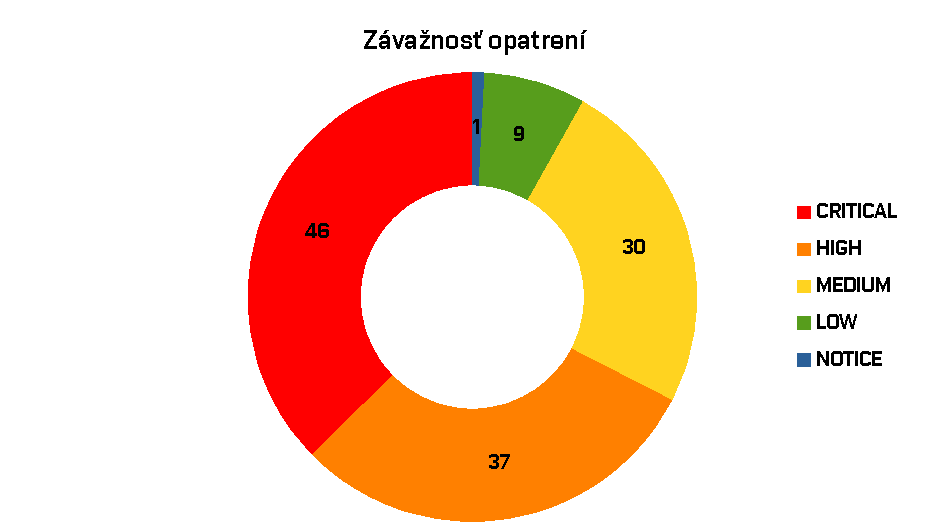
\includegraphics[scale=0.5]{obrazky/zavaznosti_graf.pdf}
%	\end{center}
%	\caption[graf_zavaznost]{Závažnosť opatrení}
%
%\end{figure}

Kybernetická bezpečnosť je bezpochyby jednou z hlavných tém 21. storočia. Útoky na infraštruktúru a systémy naberajú nielen na frekvencii, ale čo je ešte horšie na sofistikovanosti. Napriek častému zdôrazňovaniu odborníkov o kladenie čoraz väčšieho dôrazu na bezpečnosť pri návrhu, implementácii a nasadeniu, sa stále stretávame s fatálnymi dôsledkami, ktoré boli spôsobené nedostatočným venovaním pozornosti bezpečnosti. 

Problém nedostatočného zabezpečenia nie je ani tak nevedomosť základných bezpečnostných praktík administrátorov alebo programátorov, ale potreba rýchleho nasadenia systému a infraštruktúry s odložením implementácie bezpečnostných praktík na neskôr. Tieto problémy vznikajú aj pri dodatočnej implementácií nových modulov a pridaní novej infraštruktúry, kedy sa nemení celok, ale pridanie jednej časti môže výrazne ovplyvniť a zmeniť stav bezpečnosti celého systému. Z tohto dôvodu je priam žiadúce disponovať nejakým procesom alebo nástrojom na dodatočné zistenie nedostatkov a ich následnú elimináciu. Veľmi silnou motiváciou by malo byť aj to, že dôsledkom bezpečnostných nedostatkov sú globálne miliardové škody a straty reputácií firiem. 

Jednou z hlavných častí infraštruktúry, kde dochádza k významným bezpečnostným incidentom je počítačová sieť, bez ktorej by dnes informačné technológie nevedeli fungovať. Preto sa táto práca bude zaoberať práve ňou, keďže je vstupnou bránou do systémov a jej vyradením alebo zneužitím prichádzajú organizácie o finančné prostriedky, citlivé dáta a dôveru užívateľov.

Výsledkom tejto práce bude aplikácia overujúca nastavenia sieťových zariadení prevažne v lokálnej sieti, ktorá umožňuje zjednať nápravu na základe nájdených nedostatkov. Výhodou oproti existujúcim riešeniam bude otvorenosť kódu a modularita, ktorá umožní rozšírenie aplikácie na sieťové zariadenia rôznych výrobcov. Dôležitým výstupom bude taktiež zoznam bezpečnostných a prevádzkových odporučaní vychádzajúcich z rôznych štandardov a odporučaní, ktoré môžu byť v budúcnosti použité ďalšími užívateľmi aplikácie pri zostavovaní modulov pre zariadenia rôznych výrobcov. Jednou z kľúčových vlastností je bezplatnosť, keďže podľa zistení takmer polovica útokov smeruje na malé firmy, ktoré bezpečnosť často neriešia z finančnej náročnosti programov na detekciu bezpečnostných nedostatkov.    


%% Vložení souboru 'text/reseni' s popisem reseni práce
\chapter{Teoretická část studentské práce}

Teoretické zázemí studentské práce vhodně rozdělené do částí.

(Struktura navržená v~této šabloně je nejhrubší možná, po konzultaci s~vedoucím je vhodné zvolit přiléhavější.)


%% Vložení souboru 'text/vysledky' s popisem vysledků práce
\chapter{Výsledky studentské práce}

Praktická část a výsledky studenstké práce vhodně rozdělené do částí.

\section{Programové řešení}
Lorem ipsum dolor sit amet, consectetuer adipiscing elit. Nulla pulvinar eleifend sem. Integer in sapien. Etiam sapien elit, consequat eget, tristique non, venenatis quis, ante. In laoreet, magna id viverra tincidunt, sem odio bibendum justo, vel imperdiet sapien wisi sed libero. Phasellus enim erat, vestibulum vel, aliquam a, posuere eu, velit. Aliquam erat volutpat. Nullam faucibus mi quis velit \cite{sr02/2009}.

\section{Výsledky měření}
Fusce tellus odio, dapibus id fermentum quis, suscipit id erat. Fusce tellus. Morbi scelerisque luctus velit. In laoreet, magna id viverra tincidunt, sem odio bibendum justo, vel imperdiet sapien wisi sed libero. Quisque porta. Fusce suscipit libero eget elit. Nulla non lectus sed nisl molestie malesuada. Phasellus faucibus molestie nisl. Integer vulputate sem a nibh rutrum consequat. Proin mattis lacinia justo. Phasellus et lorem id felis nonummy placerat. Etiam ligula pede, sagittis quis, interdum ultricies, scelerisque eu. Cras elementum. Aenean placerat. Donec ipsum massa, ullamcorper in, auctor et, scelerisque sed, est. Aliquam ante. Integer imperdiet lectus quis justo. Vivamus ac leo pretium faucibus. Nullam faucibus mi quis velit.

\subsection{Etiam quis quam}
Neque porro quisquam est, qui dolorem ipsum quia dolor sit amet, consectetur, adipisci velit, sed quia non numquam eius modi tempora incidunt ut labore et dolore magnam aliquam quaerat voluptatem. Aliquam erat volutpat. Lorem ipsum dolor sit amet, consectetuer adipiscing elit \cite{sr02/2009,pravidla}. Nunc auctor. Neque porro quisquam est, qui dolorem ipsum quia dolor sit amet, consectetur, adipisci velit, sed quia non numquam eius modi tempora incidunt ut labore et dolore magnam aliquam quaerat voluptatem. Maecenas lorem. Maecenas libero. In laoreet, magna id viverra tincidunt, sem odio bibendum justo, vel imperdiet sapien wisi sed libero. Nullam rhoncus aliquam metus.

\subsubsection{Integer rutrum orci vestibulum}
Integer rutrum, orci vestibulum ullamcorper ultricies, lacus quam ultricies odio, vitae placerat pede sem sit amet enim. Ut enim ad minim veniam, quis nostrud exercitation ullamco laboris nisi ut aliquip ex ea commodo consequat. Fusce tellus odio, dapibus id fermentum quis, suscipit id erat. Nullam eget nisl. Nunc auctor. Etiam dui sem, fermentum vitae, sagittis id, malesuada in, quam. Fusce dui leo, imperdiet in, aliquam sit amet, feugiat eu, orci. Curabitur vitae diam non enim vestibulum interdum. Aliquam erat volutpat. Pellentesque sapien. Phasellus enim erat, vestibulum vel, aliquam a, posuere eu, velit.

\subsubsection{Eger rutrum orci westibulum}
Fusce dui leo, imperdiet in, aliquam sit amet, feugiat eu, orci. Maecenas aliquet accumsan leo. Aliquam ornare wisi eu metus. Cum sociis natoque penatibus et magnis dis parturient montes, nascetur ridiculus mus. Aliquam erat volutpat. Donec iaculis gravida nulla. Sed elit dui, pellentesque a, faucibus vel, interdum nec, diam. Temporibus autem quibusdam et aut officiis debitis aut rerum necessitatibus saepe eveniet ut et voluptates repudiandae sint et molestiae non recusandae. Nulla non arcu lacinia neque faucibus fringilla. Phasellus enim erat, vestibulum vel, aliquam a, posuere eu, velit. Praesent vitae arcu tempor neque lacinia pretium
\cite{Walter1999,Svacina1999IEEE,RajmicSysel2002}.

Aliquam erat volutpat. Quisque porta. Integer imperdiet lectus quis justo. Nullam justo enim, consectetuer nec, ullamcorper ac, vestibulum in, elit. Nullam faucibus mi quis velit. Fusce tellus. Fusce consectetuer risus a nunc. Cras pede libero, dapibus nec, pretium sit amet, tempor quis. Morbi imperdiet, mauris ac auctor dictum, nisl ligula egestas nulla, et sollicitudin sem purus in lacus
\cite{CSN_ISO_690-2011,CSN_ISO_7144-1997,CSN_ISO_31-11}.
Mauris elementum mauris vitae tortor. Neque porro quisquam est, qui dolorem ipsum quia dolor sit amet, consectetur, adipisci velit, sed quia non numquam eius modi tempora incidunt ut labore et dolore magnam aliquam quaerat voluptatem. Quisque porta. Integer vulputate sem a nibh rutrum consequat. Nulla pulvinar eleifend sem. Praesent id justo in neque elementum ultrices \cite{BiernatovaSkupa2011:CSNISO690komentar}.

Fusce suscipit libero eget elit. Integer vulputate sem a nibh rutrum consequat. Aliquam erat volutpat. Etiam neque. Nulla turpis magna, cursus sit amet, suscipit a, interdum id, felis. Nullam rhoncus aliquam metus. Etiam dui sem, fermentum vitae, sagittis id, malesuada in, quam. Nunc auctor. Nunc dapibus tortor vel mi dapibus sollicitudin. Praesent in mauris eu tortor porttitor accumsan. Nulla non arcu lacinia neque faucibus fringilla. Nullam lectus justo, vulputate eget mollis sed, tempor sed magna. Maecenas lorem. Aenean placerat. Donec vitae arcu. Maecenas lorem. Donec iaculis gravida nulla. Nulla non lectus sed nisl molestie malesuada.

Duis pulvinar. Nulla est. Duis condimentum augue id magna semper rutrum. Integer pellentesque quam vel velit. Aliquam ante. Nulla quis diam. Proin mattis lacinia justo. Aenean fermentum risus id tortor. Nunc auctor. Nullam justo enim, consectetuer nec, ullamcorper ac, vestibulum in, elit. In dapibus augue non sapien. Etiam bibendum elit eget erat. In sem justo, commodo ut, suscipit at, pharetra vitae, orci. Maecenas libero.

Nulla non lectus sed nisl molestie malesuada. Donec vitae arcu. Aenean fermentum risus id tortor. Praesent in mauris eu tortor porttitor accumsan. Nulla pulvinar eleifend sem. Duis viverra diam non justo. Integer imperdiet lectus quis justo. Pellentesque habitant morbi tristique senectus et netus et malesuada fames ac turpis egestas. In rutrum. Excepteur sint occaecat cupidatat non proident, sunt in culpa qui officia deserunt mollit anim id est laborum. Nulla non lectus sed nisl molestie malesuada. Aliquam erat volutpat. Mauris tincidunt sem sed arcu. Duis bibendum, lectus ut viverra rhoncus, dolor nunc faucibus libero, eget facilisis enim ipsum id lacus. Fusce tellus odio, dapibus id fermentum quis, suscipit id erat. In enim a arcu imperdiet malesuada. Nulla non lectus sed nisl molestie malesuada. Proin mattis lacinia justo.

Aliquam in lorem sit amet leo accumsan lacinia. Cum sociis natoque penatibus et magnis dis parturient montes, nascetur ridiculus mus. Duis sapien nunc, commodo et, interdum suscipit, sollicitudin et, dolor. Suspendisse sagittis ultrices augue. Nullam lectus justo, vulputate eget mollis sed, tempor sed magna. In convallis. Praesent id justo in neque elementum ultrices. Neque porro quisquam est, qui dolorem ipsum quia dolor sit amet, consectetur, adipisci velit, sed quia non numquam eius modi tempora incidunt ut labore et dolore magnam aliquam quaerat voluptatem.

Pellentesque pretium lectus id turpis. Nemo enim ipsam voluptatem quia voluptas sit aspernatur aut odit aut fugit, sed quia consequuntur magni dolores eos qui ratione voluptatem sequi nesciunt. Curabitur ligula sapien, pulvinar a vestibulum quis, facilisis vel sapien. Praesent dapibus. Sed elit dui, pellentesque a, faucibus vel, interdum nec, diam. Duis viverra diam non justo. Duis ante orci, molestie vitae vehicula venenatis, tincidunt ac pede. Phasellus rhoncus. Maecenas fermentum, sem in pharetra pellentesque, velit turpis volutpat ante, in pharetra metus odio a lectus. Proin pede metus, vulputate nec, fermentum fringilla, vehicula vitae, justo. Fusce aliquam vestibulum ipsum. Nullam at arcu a est sollicitudin euismod.

%Aliquam ante. Phasellus faucibus molestie nisl. Etiam ligula pede, sagittis quis, interdum ultricies, scelerisque eu. Morbi leo mi, nonummy eget tristique non, rhoncus non leo. Cum sociis natoque penatibus et magnis dis parturient montes, nascetur ridiculus mus. Morbi scelerisque luctus velit. Curabitur bibendum justo non orci. Donec quis nibh at felis congue commodo. Nullam faucibus mi quis velit. Aenean id metus id velit ullamcorper pulvinar. Pellentesque sapien. Fusce nibh. Vestibulum fermentum tortor id mi. Nullam eget nisl. Praesent vitae arcu tempor neque lacinia pretium. Proin in tellus sit amet nibh dignissim sagittis. Donec quis nibh at felis congue commodo.
%
%Nam quis nulla. Proin in tellus sit amet nibh dignissim sagittis. Nullam dapibus fermentum ipsum. Curabitur ligula sapien, pulvinar a vestibulum quis, facilisis vel sapien. Nam libero tempore, cum soluta nobis est eligendi optio cumque nihil impedit quo minus id quod maxime placeat facere possimus, omnis voluptas assumenda est, omnis dolor repellendus. Vivamus ac leo pretium faucibus. Nunc tincidunt ante vitae massa. Maecenas sollicitudin. Ut tempus purus at lorem. Nullam lectus justo, vulputate eget mollis sed, tempor sed magna. Fusce consectetuer risus a nunc. Etiam quis quam.
%
%Donec quis nibh at felis congue commodo. Sed vel lectus. Donec odio tempus molestie, porttitor ut, iaculis quis, sem. Nullam feugiat, turpis at pulvinar vulputate, erat libero tristique tellus, nec bibendum odio risus sit amet ante. Sed elit dui, pellentesque a, faucibus vel, interdum nec, diam. Cras elementum. Sed vel lectus. Donec odio tempus molestie, porttitor ut, iaculis quis, sem. Etiam neque. Integer tempor. Vivamus porttitor turpis ac leo. Nulla non arcu lacinia neque faucibus fringilla.
%
%Etiam posuere lacus quis dolor. Nemo enim ipsam voluptatem quia voluptas sit aspernatur aut odit aut fugit, sed quia consequuntur magni dolores eos qui ratione voluptatem sequi nesciunt. Nullam faucibus mi quis velit. Cum sociis natoque penatibus et magnis dis parturient montes, nascetur ridiculus mus. Phasellus faucibus molestie nisl. Maecenas ipsum velit, consectetuer eu lobortis ut, dictum at dui. Maecenas aliquet accumsan leo. Pellentesque ipsum. Donec vitae arcu. Suspendisse nisl. Morbi imperdiet, mauris ac auctor dictum, nisl ligula egestas nulla, et sollicitudin sem purus in lacus. Pellentesque ipsum. Ut enim ad minima veniam, quis nostrum exercitationem ullam corporis suscipit laboriosam, nisi ut aliquid ex ea commodi consequatur? Nam libero tempore, cum soluta nobis est eligendi optio cumque nihil impedit quo minus id quod maxime placeat facere possimus, omnis voluptas assumenda est, omnis dolor repellendus.


%% Vložení souboru 'text/zaver' se závěrem
\chapter*{Záver}
\phantomsection
\addcontentsline{toc}{chapter}{Záver}


%Buducnost - oznacovanie flase possive + komenty\\
%Dorobit backend - server \\
%co som mal spravit
%co som spravilk

% co sa nepodarili
% v skratke vyhody
% co bolo nutne nastudovat plus z kolko guidov som cerpal





Cieľom tejto diplomovej práce bol návrh a následná implementácia programu na nájdenie bezpečnostných a prevádzkových nedostatkov v sieťových zariadeniach, ako aj ich náprava pomocou generovania opravnej konfigurácie. Z tohto dôvodu bola naštudovaná problematika bezpečnosti a prevádzky sieťových zariadení a ich správna konfigurácia. Z množstva dostupnej literatúry, štandardov a odporúčaní bol vytvorený zoznam odporúčaní, na základe ktorého boli zostavované YAML moduly pre výsledný program. Tento zoznam odporúčaní bol rozšírený aj o hodnotenie závažnosti nedostatkov a priradenie prvkov zoznamu k relevantným zariadeniam v hierarchickom modely siete. Jedná sa teda o unikátne riešenie medzi bezplatnými zoznamami odporúčaní. Tento zoznam môže byť použitý aj na rozšírenie programu o podporu iných výrobcov, ale aj separátne bez akéhokoľvek využitia v programe. Vzhľadom na časovú náročnosť boli vytvorené moduly zatiaľ pre zariadenia značky Cisco. Bolo nutné zanalyzovať niekoľko stovák príkazov a ich povolených kombinácií, vytvoriť pre ne korešpondujúce regulárne výrazy a následne vytvoriť viac ako 220 YAML modulov zodpovedných za nájdenie problémov v konfiguráciách. 

Ako implementačný jazyk bol využitý Python 3.7, ktorý zaisťuje prenositeľnosť programu na viaceré platformy. Program na rozdiel od konkurencie umožňuje rozšírenie vďaka modularite aj na ďalších výrobcov sieťových zariadení a pridáva kontrolu aj pre topológie využívajúce IPv6. Taktiež rešpektuje hierarchický model siete, a teda generuje oveľa menej falošne pozitívnych správ, keďže kontroluje iba nastavenia typické pre danú vrstvu, na ktorej zariadenie operuje. Jeho výstupom je okrem iného aj prehľadná správa o kontrole zobraziteľná v PDF alebo vo webovom prehliadači. Naviac ako jediný z porovnávaných bezplatných riešení umožňuje automatické vygenerovanie nápravy, pokiaľ je to z charakteru príkazu možné. 

Napriek rôznym komplikáciám, a to hlavne neposkytnutie konfigurácií z reálnych sietí, ktoré boli vopred dohodnuté, prebehlo aj testovanie pomocou vyexportovaných konfigurácií z topológií vytvorených v nástroji GNS3.

Z pôvodného návrhu sa nepodarilo vzhľadom na časovú náročnosť celého programu implementovať vyhľadávanie zoznamu útokov a problémov aktuálne bežiacej verzie operačného systému, no počíta sa s implementáciou tejto funkcionality v budúcnosti. Ďalším rozšírením, ktoré je možné aplikovať, je pridanie podpory na ďalších výrobcov ako Juniper a HP. Využiteľné by bolo taktiež možnosť editovať záverečné správy pridaním back-endu pre HTML správy.


%% Vložení souboru 'text/literatura' se seznamem literatury
% Pro sazbu seznamu literatury použijte jednu z následujících možností

%%%%%%%%%%%%%%%%%%%%%%%%%%%%%%%%%%%%%%%%%%%%%%%%%%%%%%%%%%%%%%%%%%%%%%%%%
%1) Seznam citací definovaný přímo pomocí prostředí literatura / thebibliography

\begin{literatura}{99}
\bibitem{Milkovich3122018}
MILKOVICH, Devon. 13 Alarming Cyber Security Facts and Stats. In: \textit{Cybint} [online]. 3.12.2018 [cit. 2019-11-08]. Dostupné z: https://www.cybintsolutions.com/cyber-security-facts-stats/

\bibitem{Vyncke2008}
VYNCKE, Eric a Christopher PAGGEN. \textit{LAN switch security: What hackers know about your switches}. Indianapolis, IN: Cisco Press, 2008. ISBN :978-1-58705-256-9.	
	
\bibitem{McMillan2018}
MCMILLAN, Troy. \textit{CCNA security study guide: exam 210-260}. Indianapolis, Indiana: Sybex, a Wiley Brand, 2018. ISBN 978-111-9409-939.
	
\bibitem{Stallings2011}
STALLINGS, William. \textit{Network security essentials: applications and standards}. 4th ed. Boston: Prentice Hall, 2011. ISBN 978-0-13-610805-4.

\bibitem{Jackson2010}
JACKSON, Chris. \textit{Network security auditing}. Indianapolis, IN: Cisco Press, 2010. Cisco Press networking technology series. ISBN 978-1-58705-352-8.

\bibitem{7TVhmfuQFbsOANAz}
Guide for Conducting Risk Assessments: NIST Special Publication 800-30. In: \textit{NIST} [online]. 2012 [cit. 2019-11-08]. Dostupné z: https://nvlpubs.nist.g\
ov/nistpubs/Legacy/SP/nistspecialpublication800-30r1.pdf

	
	
	
\bibitem{Alsadeh1252015}
ALSADEH, Ahmad. Augmented SEND: Aligning Security, Privacy, and Usability. In: \textit{RIPE NCC} [online]. 12.5.2015 [cit. 2019-11-02]. Dostupné z: https://ripe70.ripe.net/presentations/67-RIPE70-SEND.pdf
\bibitem{Podermanski1222015}
PODERMAŃSKI, Tomáš a Matěj GRÉGR. Bezpečné IPv6: zkrocení zlých směrovačů. In: \textit{ROOT.CZ} [online]. 12.2.2015 [cit. 2019-11-02]. Dostupné z: https://www.root.cz/clanky/bezpecne-ipv6-zkroceni-zlych-smerovacu/
\bibitem{Khandelwal2016}
KHANDELWAL, Manjul. OSPF Security: Attacks and Defenses. In: \textit{SANOG} [online]. 2016 [cit. 2019-11-04]. Dostupné z: https://www.sanog.org/resources/sanog28/SANOG28-Tutorial\_OSPF-Security-Attacks-and-Defences-Manjul.pdf
\bibitem{Podermanski1932015}
PODERMAŃSKI, Tomáš a Matěj GRÉGR. Bezpečné IPv6: když dojde keš --- obrana. In: \textit{ROOT.CZ} [online]. 19.3.2015 [cit. 2019-11-02]. Dostupné z: https://www.root.cz/clanky/bezpecne-ipv6-kdyz-dojde-kes-obrana/
\bibitem{Podermanski1232015}
PODERMAŃSKI, Tomáš a Matěj GRÉGR. Bezpečné IPv6: když dojde keš. In: \textit{ROOT.CZ} [online]. 12.3.2015 [cit. 2019-11-02]. Dostupné z: https://www.root.cz/clanky/bezpecne-ipv6-kdyz-dojde-kes/
\bibitem{Podermanski532015}
PODERMAŃSKI, Tomáš a Matěj GRÉGR. Bezpečné IPv6: trable s multicastem. In: \textit{ROOT.CZ} [online]. 5.3.2015 [cit. 2019-11-02]. Dostupné z: https://www.root.cz/clanky/bezpecne-ipv6-trable-s-multicastem/
\bibitem{Gregr2622015}
GRÉGR, Matěj a Tomáš PODERMAŃSKI. Bezpečné IPv6: vícehlavý útočník. In: \textit{ROOT.CZ} [online]. 26.2.2015 [cit. 2019-11-02]. Dostupné z: https://www.root.cz/clanky/bezpecne-ipv6-vicehlavy-utocnik/
\bibitem{Podermanski1922015}
PODERMAŃSKI, Tomáš a Matěj GRÉGR. Bezpečné IPv6: trable s hlavičkami. In: \textit{ROOT.CZ} [online]. 19.2.2015 [cit. 2019-11-02]. Dostupné z: https://www.root.cz/clanky/bezpecne-ipv6-trable-s-hlavickami/
\bibitem{Gregr522015}
GRÉGR, Matěj a Tomáš PODERMAŃSKI. Bezpečné IPv6 : směrovač se hlásí. In: \textit{ROOT.CZ} [online]. 5.2.2015 [cit. 2019-11-02]. Dostupné z: https://www.root.cz/clanky/bezpecne-ipv6-smerovac-se-hlasi/
\bibitem{zXCpMaLbN1J7D1z2}
IPv6 First-Hop Security Configuration Guide. In: \textit{Cisco} [online]. San Jose [cit. 2019-11-02]. Dostupné z: https://www.cisco.com/c/en/us/td/docs/ios-xml/ios/ipv6\_fhsec/configuration/15-1sg/ip6f-15-1sg-book.pdf
\bibitem{Bouska2007}
BOUŠKA, Petr. \textit{Cisco IOS 12 - IEEE 802.1x a pokročilejší funkce} [online]. In: . 2007 [cit. 2019-11-02]. Dostupné z: https://www.samuraj-cz.com/clanek/cisco-ios-12-ieee-802-1x-a-pokrocilejsi-funkce/
\bibitem{yDzYjF1hoACahpg1}
MOLENAAR, René. Cisco IOS features that you should disable or restrict. In: \textit{NetworkLessons.com} [online]. [cit. 2019-11-02]. Dostupné z: https://networklessons.com/uncategorized/cisco-ios-features-that-you-should-disable-or-restrict
\bibitem{Bouska2009}
BOUŠKA, Petr. Cisco IOS 23 - Autentizace uživatele na switchi vůči Active Directory. In: \textit{SAMURAJ-cz} [online]. 2009 [cit. 2019-11-02]. Dostupné z: https://www.samuraj-cz.com/clanek/cisco-ios-23-autentizace-uzivatele-na-switchi-vuci-active-directory/
\bibitem{Barker2019}
BARKER, Elaine a Allen ROGINSKY. Transitioning the Use of Cryptographic Algorithms and Key Lengths. In: \textit{NIST} [online]. 2019 [cit. 2019-11-02]. Dostupné z: https://nvlpubs.nist.gov/nistpubs/SpecialPublications/NIST.SP.800-131Ar2.pdf
\bibitem{o31nYG4kn98wWNRS}
VYNCKE, Erik. ND on wireless links and/or with sleeping nodes. In: \textit{IETF} [online]. [cit. 2019-11-02]. Dostupné z: https://www.ietf.org/proceedings/89/slides/slides-89-v6ops-3.pdf
\bibitem{DrTLsgXv24lxeIIM}
CIS Cisco IOS 15 Benchmark. In: \textit{Center For Internet Security} [online]. 2015 [cit. 2019-11-02]. Dostupné z: https://www.cisecurity.org/benchmark/cisco/
\bibitem{Singh2018}
SINGH, Shashank. Cisco Guide to Harden Cisco IOS Devices. In: \textit{Cisco} [online]. 2018 [cit. 2019-11-02]. Dostupné z: https://www.cisco.com/c/en/us/support/docs/ip/access-lists/13608-21.html
\bibitem{Graesser2001}
GRAESSER, Dana. Cisco Router Hardening Step-by-Step. In: \textit{SANS Institute} [online]. 2001 [cit. 2019-11-02]. Dostupné z: https://www.sans.org/reading-room/whitepapers/firewalls/paper/794
\bibitem{Pilihanto2012}
PILIHANTO, Atik. A Complete Guide on IPv6 Attack and Defense. In: \textit{SANS Institute} [online]. SANS Institute, 2012 [cit. 2019-11-02]. Dostupné z: https://www.sans.org/reading-room/whitepapers/detection/paper/33904
\bibitem{Rey2016}
REY, Enno, Antonios ATLASIS a Jayson SALAZAR. MLD Considered Harmful. In: \textit{RIPE NCC} [online]. 2016 [cit. 2019-11-02]. Dostupné z: https://ripe72.ripe.net/presentations/74-ERNW\_RIPE72\_MLD\_Considered\_Harmful\_v1\_light\_web.pdf
\bibitem{Vyncke2012}
VYNCKE, Erik. IPv6 First Hop Security: the IPv6 version of DHCP snooping and dynamic ARP inspection. In: \textit{Slidde Share} [online]. 2012 [cit. 2019-11-02]. Dostupné z: https://www.slideshare.net/IKTNorge/eric-vyncke-layer2-security-ipv6-norway
\bibitem{77Eg8gGc0CKWfGBi}
IPv6 First-Hop Security Configuration Guide. In: \textit{Cisco} [online]. 2012 [cit. 2019-11-02]. Dostupné z: https://www.cisco.com/c/en/us/td/docs/ios-xml/ios/ipv6\_fhsec/configuration/15-s/ip6f-15-s-book/ip6-snooping.html
\bibitem{Gregr2011}
GREGR, Matej, Petr MATOUSEK, Miroslav SVEDA a Tomas PODERMANSKI. Practical IPv6 monitoring-challenges and techniques. In: \textit{12th IFIP/IEEE International Symposium on Integrated Network Management (IM 2011) and Workshops}. IEEE, 2011, 2011, s.~650-653. DOI: 10.1109/INM.2011.5990647. ISBN 978-1-4244-9219-0. Dostupné také z: http://ieeexplore.ieee.org/document/5990647/
\bibitem{1xYhFLUJF9lmHMC0}
PODERMAŃSKI, Tomáš a Matějj GRÉGR. \textit{Deploying IPv6 - practical problems from the campus perspective} [online]. In: . [cit. 2019-11-02].
\bibitem{Martin2016}
MARTIN, Tim. IPv6 Sys Admin Style. In: \textit{SlideShare} [online]. 2016 [cit. 2019-11-02]. Dostupné z: https://www.slideshare.net/tjmartin2020/ipv6-sysadmins-63071235
\bibitem{uYLsMtQInofenpV3}
Cisco SAFE Reference Guide. In: \textit{CIsco} [online]. San Jose, CA, 8 Júl 2018 [cit. 2019-11-02]. Dostupné z: https://www.cisco.com/c/en/us/td/docs/solutions/Enterprise/Security/SAFE\_RG/SAFE\_rg.pdf
\bibitem{JnCqiekTXFe2KIyx}
SAFE Overview Guide: Threats, Capabilities, and the Security Reference Architecture. In: \textit{Cisco} [online]. Január 2018 [cit. 2019-11-02]. Dostupné z: https://www.cisco.com/c/dam/en/us/solutions/collateral/enterprise/design-zone-security/safe-overview-guide.pdf

\bibitem{Akin2002}
AKIN, Thomas. \textit{Hardening Cisco routers}. Sebastopol: O'Reilly, 2002. ISBN 05-960-0166-5.

\bibitem{Hucaby2010}
HUCABY, Dave, Steve MCQUERRY, Andrew WHITAKER a Dave HUCABY. \textit{Cisco router configuration handbook}. 2nd ed. Indianapolis, IN: Cisco Press, 2010. ISBN 978-1-58714-116-4.
\bibitem{Satrapa2019}
SATRAPA, Pavel. \textit{IPv6: internetový protokol verze 6}. 4. aktualizované a rozšířené vydání. Praha: CZ.NIC, z.s.p.o., 2019. CZ.NIC. ISBN 978-808-8168-430.



\end{literatura}


%%%%%%%%%%%%%%%%%%%%%%%%%%%%%%%%%%%%%%%%%%%%%%%%%%%%%%%%%%%%%%%%%%%%%%%%%
%%2) Seznam citací pomocí BibTeXu
%% Při použití je nutné v TeXnicCenter ve výstupním profilu aktivovat spouštění BibTeXu po překladu.
%% Definice stylu seznamu
%\bibliographystyle{unsrturl}
%% Pro českou sazbu lze použít styl czechiso.bst ze stránek
%% http://www.fit.vutbr.cz/~martinek/latex/czechiso.tar.gz
%%\bibliographystyle{czechiso}
%% Vložení souboru se seznamem citací
%\bibliography{text/literatura}
%
%% Následující příkaz je pouze pro ukázku sazby literatury při použití BibTeXu.
%% Způsobí citaci všech zdrojů v souboru odkazy.bib, i když nejsou citovány v textu.
%\nocite{*}

%% Vložení souboru 'text/zkratky' se seznam použitých symbolů, veličin a zkratek
\begin{seznamzkratek}{KolikMista}

	\novazkratka{zkTemp}		% název
		{Šířka levého sloupce Seznamu symbolů, veličin a zkratek}								% zkratka
		{je určena šířkou parametru prostředí \texttt{seznamzkratek} (viz řádek~1 výpisu zdrojáku na~str.\,\pageref{lst:zkratky})}
											% rozvinutí zkratky

	\novazkratka{zkDummy}
		{KolikMista}
		{pouze ukázka vyhrazeného místa}

	\novazkratka{zkDSP}		% název
		{DSP}								% zkratka
		{číslicové zpracování signálů -- Digital Signal Processing}
											% rozvinutí zkratky
	%%% bsymfvz
	\novazkratka{symfvz}						% název
		{\ensuremath{f_\textind{vz}}} % symbol
		{vzorkovací kmitočet}					% popis
	%%% esymfvz

\end{seznamzkratek}


%% Začátek příloh
\prilohy

%% Vysázení seznamu příloh
\seznampriloh

%% Vložení souboru 'text/prilohy' s přílohami
\newgeometry{left=2.5cm,bottom=3.4cm, top=2.5cm}
\chapter{Kontrolný zoznam odporúčaní pre zariadenia CISCO}
\label{apendix:cisco_cmd}

\scriptsize

\begin{longtable}[!htbp]{|L{10em}L{10em}>{\fontfamily{qcr}\selectfont}L{34em}|}
	\caption{Rozpracovaná tabuľka s príkazmi na konfiguráciu zariadení od spoločnosti Cisco}
	\label{tab:cisco_table}\\ \hline
	\centering 
	
	\centering{\hspace{-3em}\vspace{1em}Útok / Problém} & Mitigácia / Nastavenie&{\fontfamily{lmr}\selectfont Príkazy}\\ \hhline{===}
	\endfirsthead
	
	
	\hline
	\centering 
	\centering{\hspace{-3em}Útok / Problém} & Mitigácia / Nastavenie&{\fontfamily{lmr}\selectfont Príkazy}\\ \hhline{===}
	\endhead
	
	
	
	\rowcolor[rgb]{ .97,  .97,  .97} Nemožná identifikácia zariadenia	&Vytvoriť hostname	&hostname $<$hostname$>$\\
	Nemožnosť vzdialeného prístupu	&Vytvoriť doménové meno	&ip domain-name $<$domain$>$\\
	
	\rowcolor[rgb]{ .97,  .97,  .97} Nepovolený prístup k manažovaniu zariadenia	&Vytvoriť a aplikovať ACL pre OOB, Telnet, SSH a pod. a zaznamenať v logu prístupy	&ip access-list standard $<$acl name$>$
	
	\hspace{0.5em}remark permit specifi ip and log
	
	\hspace{0.5em}permit $<$ip address$>$ $<$mask$>$ log-input
	
	\hspace{0.5em}remark deny other and log
	
	\hspace{0.5em}deny any log-input
	
	\vspace{0.5em}
	
	ipv6 access-list $<$acl name$>$
	
	\hspace{0.5em}remark permit specifi ip and log
	
	\hspace{0.5em}permit $<$ipv6 address$>$/$<$prefix$>$ any log-input
	
	\hspace{0.5em}remark deny other and log
	
	\hspace{0.5em}deny any any log-input
	
	\vspace{0.5em}
	{\fontfamily{lmr}\selectfont alebo v global config }
	\vspace{0.5em}
	
	login on-failure log-input
	
	login on-failure trap
	
	login on-failure
	
	login on-success log-input
	
	login on-success trap
	
	login on-success\\
	
	
	
	
	Nepovolený prístup k manažovaniu zariadenia	&Vytvoriť a aplikovať ACL pre Telnet, SSH a pod. a zaznamenať v logu prístupy	&line vty $<$num$>$ $<$num$>$
	
	\hspace{0.5em}ip access-class $<$acl name$>$ in
	
	\hspace{0.5em}ipv6 access-class $<$acl name$>$ in
	
	\vspace{0.5em}line tty $<$num$>$ $<$num$>$
	
	\hspace{0.5em}ip access-class $<$acl name$>$ in
	
	\hspace{0.5em}ipv6 access-class $<$acl name$>$ in\\
	
	
	
	
	
	\rowcolor[rgb]{ .97,  .97,  .97}Neautorizovaný prístup cez nepoužívané a nezabezpečené protokoly na manažment zariadení	&Vypnúť nepoužívané protokoly na prístup k manažovaniu zariadení (telnet a pod.)	&line aux 0
	
	\hspace{0.5em}no exec
	
	\hspace{0.5em}transport input none\\
	
	
	
	
	Prístup bez požadovaných prístupových údajov	&Nakonfigurovanie protokolov na manažment zariadení, aby požadovali prístupové údaje (telnet a pod.)	&line vty $<$num$>$ $<$num$>$
	\hspace{0.5em}password
	
	\hspace{0.5em}login | login local
	
	\vspace{0.5em}line tty $<$num$>$ $<$num$>$
	
	\hspace{0.5em}password
	
	\hspace{0.5em}login | login local
	
	\vspace{0.5em}
	line con $<$num$>$
	
	\hspace{0.5em}password
	
	\hspace{0.5em}login | login local
	
	\vspace{0.5em}line aux $<$num$>$
	
	\hspace{0.5em}password
	
	\hspace{0.5em}login | login local\\
	
	
	
	
	\rowcolor[rgb]{ .97,  .97,  .97}Nepoužívanie zabezpečeného protokolu na manažment zariadení môže viesť k odposluchu	&Zapnutie SSH	&line vty $<$num$>$ $<$num$>$
	
	\hspace{0.5em}login local
	
	\hspace{0.5em}transport input ssh\\
	
	
	
	Nebezpečná verzia 1 protokolu SSH	&SSH verzia 2	&ip ssh version 2\\
	
	
	
	
	\rowcolor[rgb]{ .97,  .97,  .97}Dlhé neaktívne sedenie môže byť zneužité alebo aj fyzický prístup útočníka k aktívnemu sedeniu môže viesť k zmene konfigurácie	&SSH čas vypršania sedenia	&ip ssh timeout $<$timeout seconds$>$\\
	
	
	
	
	Útok na krátky RSA kľúč	&Dĺžka RSA kľúča minimálne 2048 bitov	&crypto key generate rsa modulus 2048\\
	
	
	
	
	\rowcolor[rgb]{ .97,  .97,  .97}Hádanie hesla k RSA kľúču	&SSH maximálny počet neúspešných pokusov	&ip 
	ssh authentication-retries $<$max num$>$\\
	
	
	
	
	Útok hrubou silou na zistenie prihlasovacích údajov	&Špecifikovať čas po ktorý nie je možné po N pokusoch sa prihlásiť	&login block-for 60 attempts 3 within 30\\
	
	
	
	
	\rowcolor[rgb]{ .97,  .97,  .97} Prihlásenie na zariadenie nie je možné kvôli zablokovaniu pre príliš veľa neúspešných pokusov	&Povolenie prístupu administrátorovi na základe IP adresy, keď je protokol na manažovanie zariadení nedostupný kvôli DOS útoku	&login quiet-mode access-class $<$acl name$>$\\
	
	
	
	Možné prihlásenie do zariadenia cez telnet keď je prítomné SSH	&Zakázať telnet ak je SSH aktívne	&line vty $<$num$>$ $<$num$>$
	
	\hspace{0.5em}no transport input all
	
	\hspace{0.5em}no transport input telnet
	\vspace{0.5em}
	
	line tty $<$num$>$ $<$num$>$
	
	\hspace{0.5em}no transport input all
	
	\hspace{0.5em}no transport input telnet
	\vspace{0.5em}
	
	line con $<$num$>$
	
	\hspace{0.5em}no transport input all
	
	\hspace{0.5em}no transport input telnet
	\vspace{0.5em}
	
	line aux $<$num$>$
	
	\hspace{0.5em}no transport input all
	
	\hspace{0.5em}no transport input telnet\\
	
	
	
	
	\rowcolor[rgb]{ .97,  .97,  .97} Útočník nie je informovaný o právnych následkoch	&Právne upozornenie pri prístupe k zariadeniu	&banner motd
	
	banner login
	
	banner exec\\
	
	
	
	Dlhé neaktívne sedenie môže byť zneužité alebo aj fyzický prístup útočníka k aktívnemu sedeniu môže viesť k zmene konfigurácie	&Čas vypršania sedenia pre protokol na manažovanie zariadení	&line vty $<$num$>$ $<$num$>$
	
	exec-timeout 5
	\vspace{0.5em}
	
	line tty $<$num$>$ $<$num$>$
	
	\hspace{0.5em}exec-timeout 5
	\vspace{0.5em}
	
	line con $<$num$>$
	
	\hspace{0.5em}exec-timeout 5
	\vspace{0.5em}
	
	line aux $<$num$>$
	
	\hspace{0.5em}exec-timeout 5\\
	
	
	
	
	\rowcolor[rgb]{ .97,  .97,  .97} Možnosť prečítať heslá z uniknutých konfigurácií	&Zašifrovanie hesiel v otvorenej podobe	&service password-encryption\\
	
	
	
	
	Nepovolená zmena konfigurácie zariadenia	&Vytvorenie hesla na editovanie konfigurácie zariadenia	&enable secret $<$secret password$>$\\
	
	
	
	
	\rowcolor[rgb]{ .97,  .97,  .97} Nepovolená zmena konfigurácie zariadenia	&Vytvorenie hesla na editovanie konfigurácie zariadenia	&no enable password $<$password$>$\\
	
	
	
	Nepovolený prístup k manažmentu konfigurácie zariadenia	&Lokálne zabezpečené účty	&username secret $<$username$>$ $<$secret password$>$\\
	
	
	
	\rowcolor[rgb]{ .97,  .97,  .97} Nepovolený prístup k manažmentu konfigurácie zariadenia	&Lokálne zabezpečené účty	&no username password  $<$username$>$ $<$password$>$\\
	
	
	
	Centrálna správa prihlásení a dohľadateľnosť zmien v konfigurácií	&Definovanie a povolenie AAA serveru na prihlásenie a definovanie záložného prihlásenia	&aaa new-model
	
	radius server $<$radius server name$>$
	
	\hspace{0.5em}address ipv4 $<$ip adddress$>$ / address ipv6 $<$ipv6 adddress$>$
	
	\hspace{0.5em}key $<$password$>$
	\vspace{0.5em}
	
	{\fontfamily{lmr}\selectfont alebo}
	
	\vspace{0.5em}
	radius-server host $<$ip adddress$>$
	
	radius-server key $<$password$>$
	
	\vspace{0.5em}
	
	aaa group server radius $<$radius group$>$
	
	\hspace{0.5em}server name $<$radius server name$>$
	
	aaa authentication login default / $<$radius login$>$ group 
	
	\hspace{0.5em}$<$radius group$>$ local enable
	
	line tty $<$num$>$ $<$num$>$
	
	\hspace{0.5em}login authentication default / $<$radius login$>$
	
	line vty $<$num$>$ $<$num$>$
	
	\hspace{0.5em}login authentication default / $<$radius login$>$
	
	line con $<$num$>$
	
	\hspace{0.5em}login authentication default / $<$radius login$>$
	
	line aux $<$num$>$
	
	
	\hspace{0.5em}login authentication default / $<$radius login$>$\\
	
	
	
	
	\rowcolor[rgb]{ .97,  .97,  .97} Centrálna správa prihlásení a dohľadateľnosť zmien v konfigurácií	&Definovanie a povolenie AAA serveru na prihlásenie a definovanie záložného prihlásenia	&aaa new-model
	
	tacacs server $<$tacacs server name$>$
	
	\hspace{0.5em}address ipv4 $<$ip adddress$>$ / address ipv6 $<$ipv6 adddress$>$
	
	\hspace{0.5em}key $<$password$>$
	\vspace{0.5em}
	
	{\fontfamily{lmr}\selectfont alebo}
	
	\vspace{0.5em}
	tacacs-server host $<$ip adddress$>$
	
	tacacs-server key $<$password$>$
	
	\vspace{0.5em}
	
	aaa group server tacacs $<$tacacs group$>$
	
	\hspace{0.5em}server name $<$tacacs server name$>$
	
	aaa authentication login default / $<$tacacs login$>$ group 
	
	\hspace{0.5em}$<$tacacs group$>$ local enable
	
	line tty $<$num$>$ $<$num$>$
	
	\hspace{0.5em}login authentication default / $<$tacacs login$>$
	
	line vty $<$num$>$ $<$num$>$
	
	\hspace{0.5em}login authentication default / $<$tacacs login$>$
	
	line con $<$num$>$
	
	\hspace{0.5em}login authentication default / $<$tacacs login$>$
	
	line aux $<$num$>$
	
	
	\hspace{0.5em}login authentication default / $<$tacacs login$>$\\
	
	
	
	
	Centrálna správa prihlásení a dohľadateľnosť zmien v konfigurácií	&Definovanie a povolenie AAA serveru na editáciu konfigurácií a definovanie záložného prihlásenia	&aaa authentication enable default group 
	
	\hspace{0.5em}$<$radius group$>$ enable\\
	
	
	
	
	\rowcolor[rgb]{ .97,  .97,  .97} Centrálna správa prihlásení a dohľadateľnosť zmien v konfigurácií	&Definovanie a povolenie AAA serveru na editáciu konfigurácií a definovanie záložného prihlásenia	&no aaa authentication enable default enable\\
	
	
	
	
	Hádanie prístupových údajov	&Definovanie maximálneho počtu neúspešných pokusov o prihlásenie a následné zablokovanie účtu	&aaa authentication attempts login 3\\
	
	
	
	
	\rowcolor[rgb]{ .97,  .97,  .97} Prihlásenie bez prihlasovacích údajov	&Zakázať záložné prihlásenie bez poskytnutia autentizačných prostriedkov	&{\fontfamily{lmr}\selectfont vyhnúť sa} aaa authentication login.*none.*\\
	
	
	
	
	AAA používa primárne lokálne účty namiesto centralizovaných na serveri	&AAA nesmie používať ako prvú možnosť prihlásenia lokálny účet 	&{\fontfamily{lmr}\selectfont vyhnúť sa} authentication login default local\\
	
	
	
	
	\rowcolor[rgb]{ .97,  .97,  .97} Používateľ prihlásený do zariadenia môže spúšťať akékoľvek príkazy	&Nastavenie AAA autorizácie pre spúšťanie príkazov. V prípade výpadku AAA serveru, bude užívateľ odhlásený a následne prihlásený podľa  záložného prihlásenia, aby mu nebolo pridelené vysoké oprávnenie umožňujúce vykonávať príkazy, na ktoré nemá právo	&aaa authorization exec $<$radius login$>$ group $<$radius group$>$ 
	
	\hspace{0.5em}local if-authenticated\\
	
	
	
	
	Používateľ prihlásený do zariadenia môže spúšťať akékoľvek príkazy	&Nastavenie AAA autorizácie pre spúšťanie príkazov. V prípade výpadku AAA serveru, bude užívateľ odhlásený a následne prihlásený podľa  záložného prihlásenia, aby mu nebolo pridelené vysoké oprávnenie umožňujúce vykonávať príkazy, na ktoré nemá právo	&aaa authorization commands 15 $<$radius login$>$ group
	
	\hspace{0.5em} $<$radius group$>$ local if-authenticated \\
	
	
	
	
	\rowcolor[rgb]{ .97,  .97,  .97} Administrátor vloží zlý príkaz a po čase je ho nemožné dohľadať a zjednať nápravu	&Nastavenie AAA účtovania respektíve logovania pripojení a vykonaných príkazov	&aaa accounting connection
	
	aaa accounting commands
	
	aaa accounting exec\\
	
	
	
	
	Odpočúvanie SNMP verzie 1 a 2c	&Použitie SNMP verzie 3 pokiaľ je SNMP používané	&no snmp-server community
	no snmp-server host  version 1/2c
	
	snmp-server group $<$group name$>$ v3 priv \\
	
	
	
	
	\rowcolor[rgb]{ .97,  .97,  .97} AAA zdrojové rozhranie nie je rovnaké pri každom reštarte	&Definovanie loopback zdrojového rozhrania pre AAA	&ip radius source interface loopback $<$id$>$
	
	ip tacacs source interface loopback $<$id$>$\\
	
	
	
	
	Modifikovanie konfigurácie pomocou SNMP	&Obmedzenie SNMP iba na čítanie	&snmp-server view $<$view name$>$ iso included
	
	snmp-server group $<$group name$>$ v3 priv read $<$view name$>$\\
	
	
	
	
	\rowcolor[rgb]{ .97,  .97,  .97} Neoprávnený prístup k SNMP informáciám	&Obmedzenie SNMP iba pre vybrané IP adresy	&ip access-list standard $<$acl name$>$
	
	\hspace{0.5em}remark permit only this IP 
	
	\hspace{0.5em}permit $<$ip address$>$ $<$wildcard mask$>$
	
	\hspace{0.5em}deny any log-input
	\vspace{0.5em}
	
	ipv6 access-list $<$acl name$>$
	
	\hspace{0.5em}remark permit only this IP 
	
	\hspace{0.5em}permit $<$ipv6 address$>$/$<$prefix$>$ any
	
	\hspace{0.5em}remark deny other
	
	\hspace{0.5em}deny any any log-input
	
	snmp-server group $<$group name$>$ v3 priv read $<$view name$>$  access $<$acl name$>$\\
	
	
	
	
	Administrátor nemá povedomie o problémoch na zariadení	&Povolenie asynchrónnych správ SNMP TRAP	&snmp-server host $<$ip adddress$>$ traps version 3 priv $<$user$>$
	
	snmp-server host $<$ip adddress$>$ version 3 priv $<$user$>$\\
	
	
	
	
	\rowcolor[rgb]{ .97,  .97,  .97} Odpočúvanie SNMP sedenie z dôvodu slabého šifrovania a hashovacej  funkcie	&Vytvorenie SNMP verzie 3 užívateľa s minimálnym šifrovaním AES 128 bit a hashovacou funkciou SHA	&snmp-server user $<$user$>$ $<$group name$>$ v3 auth sha 
	
	\hspace{0.5em}$<$password$>$ pri aes 128 $<$password$>$\\
	
	
	
	
	Sťažená identifikácia SNMP správ z rôznych IP	&Definovanie lokácie SNMP serveru	&snmp-server location $<$location$>$\\
	
	
	
	
	\rowcolor[rgb]{ .97,  .97,  .97} SNMP zdrojové rozhranie nie je rovnaké pri každom reštarte	& Definovanie loopback zdrojového rozhrania pre SNMP	&snmp-server trap-source loopback $<$id$>$\\
	
	
	
	
	Zmeny názvov rozhraní medzi reštartami a nemožnosť monitorovanie pomocou SNMP	&SNMP statické nemenné meno rozhrania aj po reštarte zariadenia	&snmp-server ifindex persist\\
	
	
	
	
	\rowcolor[rgb]{ .97,  .97,  .97} Administrátor nemá povedomie o problémoch na zariadení	&Povolenie logovania protokolom SYSLOG a špecifikovanie IP adresy SYSLOG serveru	&logging on
	logging host $<$ip adddress$>$\\
	
	
	
	
	Neprijímanie všetkých dôležitých incidentov na zariadení z protokolu SYSLOG	&Špecifikovanie dôležitosti oznámení SYSLOG na INFORMATIONAL	&logging trap informational\\
	
	
	
	
	\rowcolor[rgb]{ .97,  .97,  .97} SYSLOG zdrojové rozhranie nie je rovnaké pri každom reštarte	& Definovanie loopback zdrojového rozhrania pre SYSLOG	&logging source-interface loopback $<$id$>$\\
	
	
	
	Nedostatočné a neštandardné formáty času pri logovacích správach	&Definovanie formátu času pre logovacie a ladiace výstupy	&service timestamp log datetime
	
	service timestamp debug datetime\\
	
	
	
	
	\rowcolor[rgb]{ .97,  .97,  .97} Administrátor nevidí dôležité incidenty pri prihlásení a konfigurovaní cez konzolu	&Vypisovanie SYSLOG správ CRITICAL a dôležitejších do terminálu	&logging console critical\\
	
	
	
	
	Malá vyrovnávacia pamäť pre SYSLOG je dôvodom zahadzovanie správ	&Definovanie veľkosti SYSLOG buffera dôležitosti oznámení na INFORMATIONAL	&logging buffered 64000 6\\
	
	
	
	
	\rowcolor[rgb]{ .97,  .97,  .97} Neprístupný SYSLOG server spôsobuje zahadzovanie dôležitých syslog správ	&Definovanie dočasného úložiska SYSLOG správ v prípade nedostupnosti servera	&logging persistent url flash:/syslog\\
	
	
	
	
	Skenovanie a zistenie informácií o sieti za pomoci protokolu CDP a využitie bezpečnostných chýb	&Zakázanie protokolu CDP	&no cdp run
	
	
	interface $<$interface name$>$ $<$interface id$>$ 
	
	\hspace{0.5em}no cdp enable\\
	
	
	
	
	\rowcolor[rgb]{ .97,  .97,  .97} Skenovanie a zistenie informácií o sieti za pomoci protokolu LLDP a využitie bezpečnostných chýb	&Zakázanie protokolu LLDP	&no lldp run
	
	interface $<$interface name$>$ $<$interface id$>$	
	
	\hspace{0.5em}no lldp receive 
	
	\hspace{0.5em}no lldp transmit\\
	
	
	
	
	Nekonzistencia časov v logoch a problém pričlenenia logov k relevantným incidentom	&Nastavenie NTP serveru pre aktuálny čas v logoch	&ntp server $<$ip adddress$>$\\
	
	
	
	
	\rowcolor[rgb]{ .97,  .97,  .97} Pripojenie servera s rovnakou IP adresou, ale falošným časom	&Nastavenie NTP autentizácie	&ntp authenticate
	
	ntp authentication-key 1 md5 $<$password$>$
	
	trusted-key 1\\
	
	
	
	
	NTP zdrojové rozhranie nie je rovnaké pri každom reštarte	& Definovanie loopback zdrojového rozhrania pre NTP	&ntp source loopback $<$id$>$\\
	
	
	
	
	\rowcolor[rgb]{ .97,  .97,  .97}Väčšia bezpečnosť (pub/priv key) NTP a podpora IPv6	&Použitie NTP verzie 4	&ntp server $<$ip adddress$>$ version 4\\
	
	
	
	Falošný čas od podvrhnutého NTP zdroja	&Nastavenie NTP peer s inými sieťovými zariadeniami na krížovú validáciu času a záložný zdroj času	&ntp peer $<$ip adddress$>$
	
	ip access-list standard $<$acl name$>$
	
	\hspace{0.5em}remark permit only this IP 
	
	\hspace{0.5em}permit $<$ip adddress$>$ $<$wildcard mask$>$
	
	\hspace{0.5em}remark deny other 
	
	\hspace{0.5em}deny any log-input
	
	ntp access-group serve-only $<$acl name$>$
	
	interface $<$interface name$>$ $<$interface id$>$
	
	\hspace{0.5em}ntp disable\\
	
	
	
	
	\rowcolor[rgb]{ .97,  .97,  .97} Útočník s fyzickým prístupom k zariadeniu alebo portu môže odpočúvať alebo posielať škodlivý obsah	&Explicitne zakázať nepoužívané porty	&interface $<$interface name$>$ $<$interface id$>$
	
	\hspace{0.5em}shutdown\\
	
	
	
	
	Zdrojové rozhranie pre management a control protokoly	&Vytvoriť Loopback rozhranie s IP adresou	&interface loopback $<$id$>$
	
	\hspace{0.5em}ip address $<$ip paddress$>$\\
	
	
	
	
	\rowcolor[rgb]{ .97,  .97,  .97} Identifikácia pravidla v ACL	&Popis každého pravidla v ACL pre lepšiu identifikáciu	&ip access-list standard $<$acl name$>$
	
	\hspace{0.5em}remark Deny SNMP from VLAN 20
	
	\hspace{0.5em}deny ip $<$ip address$>$ $<$wildcard mask$>$
	\vspace{0.5em}
	
	ipv6 access-list $<$acl name$>$
	
	\hspace{0.5em}remark Deny SNMP from VLAN 20
	
	\hspace{0.5em}deny $<$ipv6 address$>$ $<$prefix$>$ any\\
	
	
	
	
	Identifikácia rozhrania	&Popis každého rozhrania	&interface $<$interface name$>$ $<$interface id$>$
	
	\hspace{0.5em}description PRODUCTION\_SERVER\\
	
	
	
	
	\rowcolor[rgb]{ .97,  .97,  .97}SSH zdrojové rozhranie nie je rovnaké pri každom reštarte	& Definovanie loopback zdrojového rozhrania pre SSH	&ip ssh source-interface loopback $<$id$>$\\
	
	
	
	
	DOS útok na štandardný SSH port 22	&Špecifikovanie iného portu pre SSH ako štandardného alebo aplikovanie port knocking	&ip ssh port 2223
	
	\vspace{0.5em}
	{\fontfamily{lmr}\selectfont alebo}
	\vspace{0.5em}
	
	ip access-list extended $<$acl name$>$
	
	\hspace{0.5em}remark *** KNOCK ***
	
	\hspace{0.5em}permit udp any any eq 65535 log-input
	
	\hspace{0.5em}remark *** TRUSTED ***
	
	\hspace{0.5em}permit tcp any any established
	
	\hspace{0.5em}remark *** DENIED ***
	
	\hspace{0.5em}deny   tcp any any log input
	
	\hspace{0.5em}remark *** PERMITED ***
	
	\hspace{0.5em}permit ip any any
	
	
	interface $<$interface name$>$ $<$interface id$>$
	
	\hspace{0.5em}ip access-group $<$acl name$>$
	
	\hspace{0.5em}ipv6 traffic-filter $<$acl name$>$
	
	event manager environment $<$env name$>$ $<$acl name$>$
	
	event manager applet KNOCK
	
	\hspace{0.5em}event syslog pattern "\%SEC-6-IPACCESSLOGP: list \$KNOCK\_ACL
	
	\hspace{1em}permitted *"
	
	\hspace{0.5em}action 1.0 regexp "[0-9]+$\backslash$.[0-9]+$\backslash$.[0-9]+$\backslash$.[0-9]+" \$\_syslog\_msg ADDR
	
	\hspace{0.5em}action 1.1 regexp "$\backslash$([0-9]+$\backslash$)," "\$\_syslog\_msg" PORT
	
	\hspace{0.5em}action 1.2 regexp "[0-9]+" "\$PORT" PORT 
	
	\hspace{0.5em}action 2.0 syslog msg "Received a knock from \$ADDR on port \$PORT..."
	
	\hspace{0.5em}action 2.1 syslog msg "Adding \$ADDR to the \$KNOCK\_ACL ACL"
	
	\hspace{0.5em}action 3.0 cli command "enable"
	
	\hspace{0.5em}action 3.1 cli command "configure terminal"
	
	\hspace{0.5em}action 3.2 cli command "ip access-list extended \$KNOCK\_ACL"
	
	\hspace{0.5em}action 3.3 cli command "1 permit tcp host \$ADDR any eq 22"
	
	\hspace{0.5em}action 4.0 WAIT 15
	
	\hspace{0.5em}action 5.0 syslog msg "Removing \$ADDR to the \$KNOCK\_ACL ACL"
	
	\hspace{0.5em}action 6.0 cli command "no permit tcp host \$ADDR any eq 22"
	
	\hspace{0.5em}action 6.1 cli command "exit"\\
	
	
	
	\rowcolor[rgb]{ .97,  .97,  .97}Nepovolený prístup k manažmentu konfigurácie zariadenia	&Vypnutie odchádzajúcich spojení pre protokoly na manažment zariadení pokiaľ sa nepoužívajú (telnet a pod.)	&line vty $<$num$>$ $<$num$>$
	
	\hspace{0.5em}transport output none
	
	line tty $<$num$>$ $<$num$>$
	
	\hspace{0.5em}transport output none
	
	line con $<$num$>$
	
	\hspace{0.5em}transport output none
	
	line aux $<$num$>$
	
	\hspace{0.5em}transport output none\\
	
	
	
	
	
	Odpočúvanie konfigurácií zariadení pri zálohe	&Zapnutie zabezpečenej zálohy na server (SFTP, SCP)	&ip scp server enable
	
	copy startup-config scp://$<$username$>$@$<$ip address$>$/backup\\
	
	
	
	
	\rowcolor[rgb]{ .97,  .97,  .97}Vymazanie konfigurácie	&Zapnutie ochrany pred výmazom konfigurácie	&secure boot config\\
	
	
	
	Možnosť urobiť diff zmien konfigurácií a jej návrat	&Periodické zálohovanie konfigurácie a logovanie jej zmien	&archive
	write-memory
	
	time-period $<$num$>$
	
	log changes
	
	log config
	
	logging enable
	
	logging size $<$num$>$
	
	
	hidekeys
	
	notify syslog
	
	maximum $<$num$>$\\
	
	
	
	
	\rowcolor[rgb]{ .97,  .97,  .97} DOS útok alebo pokus o prístup k tomu, čo nie je povolené	&Logovanie pravidiel zahodenia paketov v ACL	&ip access-list standard $<$acl name$>$
	
	\hspace{0.5em}deny any log-input
	
	ipv6 access-list $<$acl name$>$
	
	\hspace{0.5em}deny any any log-input\\
	
	
	
	
	Nízky stav voľnej pamäte	&Nastavenie notifikácie pri dochádzaní pamäte	&memory free low-watermark processor $<$threshold$>$
	
	memory free low-watermark io $<$threshold$>$\\
	
	
	
	
	\rowcolor[rgb]{ .97,  .97,  .97}Logovacie správy nemôžu byť zaznamenané kvôli nedostatku pamäte	&Rezervovanie pamäte pre kritické notifikácie pri nedostatku pamäte	&memory reserve critical $<$value$>$ \\
	
	
	
	
	Vysoké zaťaženie CPU	&Nastavenie notifikácie vysokom zaťažení CPU	&snmp-server enable traps cpu threshold
	
	snmp-server host $<$ip adddress$>$ version 3 priv $<$user$>$ cpu
	
	process cpu threshold type $<$type$>$ rising 
	
	\hspace{0.5em}$<$percentage$>$ interval $<$seconds$>$
	
	process cpu statistics limit entry-percentage\\
	
	
	
	\rowcolor[rgb]{ .97,  .97,  .97} Vysoké zaťaženie zariadenia spôsobilo nemožnosť prihlásenia k nemu	&Rezervovanie pamäte pre protokoly na manažment zariadení pri nedostatku pamäte	&memory reserve console 4096\\
	
	
	
	Pretečenie pamäte	&Povoliť mechanizmy na detekciu pretečenia pamäte	&exception memory ignore overflow io
	
	exception memory ignore overflow processor
	
	exception crashinfo maximum files $<$number-of-files$>$\\
	
	
	
	
	\rowcolor[rgb]{ .97,  .97,  .97}Načítanie škodlivej konfigurácie zo siete počas bootovania	&Vypnutie načítania operačného systému alebo konfigurácie zo siete pokiaľ to nie je nutné	&no boot network
	no service config\\
	
	
	
	
	Proxy ARP môže viesť k obídeniu PVLAN a rozširuje broadcast doménu	&Vypnutie Proxy ARP	&no proxy-arp\\
	
	
	
	\rowcolor[rgb]{ .97,  .97,  .97}DOS útok na stanicu, cez ktorú bola špecifikovaná cesta a teda nemožnosť komunikácie s koncovým bodom. Alebo zosnovanie MITM útoku	&Vypnutie IP source routing	&no ip source-route\\
	
	
	
	
	DOS útok pomocou podvrhnutej IP adresy alebo vzdialený útok na smerovací protokol	&Zapnutie reverse path forwarding strict/loose mode	&ip verify unicast source reachable-via rx\\
	
	
	
	\rowcolor[rgb]{ .97,  .97,  .97} Nepoužívané, staré a nezabezpečené služby môžu byť použité na škodlivé účely	&Vypnutie nepoužívaných služieb z bezpečnostných dôvodov a na šetrenie CPU a pamäte 	&no ip bootp server\\
	
	
	
	
	Nepoužívané, staré a nezabezpečené služby môžu byť použité na škodlivé účely	&Vypnutie nepoužívaných služieb z bezpečnostných dôvodov a na šetrenie CPU a pamäte 	&no service pad\\
	
	
	
	
	\rowcolor[rgb]{ .97,  .97,  .97} Nepoužívané, staré a nezabezpečené služby môžu byť použité na škodlivé účely	&Vypnutie nepoužívaných služieb z bezpečnostných dôvodov a na šetrenie CPU a pamäte 	&no ip identd\\
	
	
	
	Nepoužívané, staré a nezabezpečené služby môžu byť použité na škodlivé účely	&Vypnutie nepoužívaných služieb z bezpečnostných dôvodov a na šetrenie CPU a pamäte 	&no vstack\\
	
	
	
	\rowcolor[rgb]{ .97,  .97,  .97} Nepoužívané, staré a nezabezpečené služby môžu byť použité na škodlivé účely	&Vypnutie nepoužívaných služieb z bezpečnostných dôvodov a na šetrenie CPU a pamäte 	&no ip http server
	
	no ip http secure server\\
	
	
	
	Nepoužívané, staré a nezabezpečené služby môžu byť použité na škodlivé účely	&Vypnutie nepoužívaných služieb z bezpečnostných dôvodov a na šetrenie CPU a pamäte 	&no service tcp-small-server\\
	
	
	
	
	\rowcolor[rgb]{ .97,  .97,  .97} Nepoužívané, staré a nezabezpečené služby môžu byť použité na škodlivé účely	&Vypnutie nepoužívaných služieb z bezpečnostných dôvodov a na šetrenie CPU a pamäte 	&no service udp-small-server\\
	
	
	
	Nepoužívané, staré a nezabezpečené služby môžu byť použité na škodlivé účely	&Vypnutie nepoužívaných služieb z bezpečnostných dôvodov a na šetrenie CPU a pamäte 	&no service finger\\
	
	
	
	
	\rowcolor[rgb]{ .97,  .97,  .97} Nepoužívané, staré a nezabezpečené služby môžu byť použité na škodlivé účely	&Vypnutie nepoužívaných služieb z bezpečnostných dôvodov a na šetrenie CPU a pamäte 	&interface $<$interface name$>$ $<$interface id$>$
	
	\hspace{0.5em} no mop enabled\\
	
	
	
	Nepoužívané, staré a nezabezpečené služby môžu byť použité na škodlivé účely	&Vypnutie nepoužívaných služieb z bezpečnostných dôvodov a na šetrenie CPU a pamäte 	&no ip domain lookup\\
	
	
	
	\rowcolor[rgb]{ .97,  .97,  .97} Útočník môže zistiť, že IP adresa, na ktorú skúšal ping je nesprávna	&Vypnutie správ ICMP Unreachable	&interface $<$interface name$>$ $<$interface id$>$
	
	\hspace{0.5em}no ip unreachables\\
	
	
	
	
	Útočník môže zistiť masku podsiete pomocou ICMP Mask reply	&Vypnutie správ ICMP Mask reply	&interface $<$interface name$>$ $<$interface id$>$
	
	\hspace{0.5em}no ip mask-reply\\
	
	
	
	
	\rowcolor[rgb]{ .97,  .97,  .97} Umožňuje DOS Smurf útok, mapovanie siete pomocou ping na broadcast adresu vzdialenej siete	&Vypnutie ICMP echo správ na broadcast adresu, vypnutie directed broadcasts	&interface $<$interface name$>$ $<$interface id$>$
	
	\hspace{0.5em}no ip directed-broadcast\\
	
	
	
	
	Útočník môže zistiť smerovacie informácie alebo vyťažiť CPU	&Vypnutie správ ICMP Redirects	&interface $<$interface name$>$ $<$interface id$>$
	
	\hspace{0.5em}no ip redirects\\
	
	
	
	\rowcolor[rgb]{ .97,  .97,  .97} Nekonzistencia konfiguračných súborov pri zmenách konfigurácie viac ako jedným administrátorom	&Povoliť súčasne iba jednému administrátorovi vykonávanie zmien v konfigurácii	&configuration mode exclusive auto\\
	
	
	
	
	Problém identifikácie SYSLOG správ s rovnakou časovou značkou	&Pridanie sekvenčného čísla ku každej syslog správe	&service sequence-numbers\\
	
	
	
	
	\rowcolor[rgb]{ .97,  .97,  .97} Nemožnosť prihlásenia pri zaseknutom TCP spojení	&Terminovanie zaseknutého TCP spojenia	&service tcp-keepalives-in
	
	service tcp-keepalives-out\\
	
	
	
	
	Vloženie a manipulácia so smerovacími informáciami	&Autentizácia smerovacích protokolov (nie heslá v otvorenej podobe)	&router bgp $<$as number$>$
	
	\hspace{0.5em}neighbor $<$ip address$>$ password $<$password$>$  \\
	
	
	
	
	\rowcolor[rgb]{ .97,  .97,  .97} Vloženie a manipulácia so smerovacími informáciami	&Autentizácia smerovacích protokolov (nie heslá v otvorenej podobe)	&key chain $<$chain name$>$
	
	\hspace{0.5em}key$<$id$>$
	
	\hspace{1em}key-string $<$password$>$
	
	interface $<$interface name$>$ $<$interface id$>$
	
	\hspace{0.5em}ip authentication mode eigrp $<$as$>$ md5
	
	\hspace{0.5em}ip authentication keyc-chain eigrp $<$as$>$ $<$chain name$>$
	
	\hspace{0.5em}ipv6 authentication mode eigrp $<$as$>$ md5
	
	\hspace{0.5em}ipv6 authentication keyc-chain eigrp $<$as$>$ $<$chain name$>$\\
	
	
	
	
	Vloženie a manipulácia so smerovacími informáciami	&Autentizácia smerovacích protokolov (nie heslá v otvorenej podobe)	&key chain $<$chain name$>$
	
	\hspace{0.5em}key$<$id$>$
	\hspace{1em}key-string $<$password$>$
	
	router ospf $<$process id$>$
	
	\hspace{0.5em}area $<$ared id$>$ authentication message-digest
	
	\hspace{0.5em}area $<$area id$>$ authentication key-chain $<$chain name$>$
	
	ipv6 router ospf $<$process id$>$
	
	\hspace{0.5em}area $<$area id$>$ authentication message-digest
	
	interface $<$interface name$>$ $<$interface id$>$
	
	\hspace{0.5em}ip ospf message-digest-key $<$key id$>$ md5|sha $<$password$>$
	
	\hspace{0.5em}ip ospf authentication message-digest
	
	\hspace{0.5em}ospfv3 authentication md5 0 2757613409476813242031209727
	
	\hspace{0.5em}no ip ospf authentication-key OPENKEY\\
	
	
	
	
	\rowcolor[rgb]{ .97,  .97,  .97} Vloženie a manipulácia so smerovacími informáciami	&Autentizácia smerovacích protokolov (nie heslá v otvorenej podobe)	&key chain $<$chain name$>$
	
	\hspace{0.5em}key $<$id$>$
	
	\hspace{1em}key-string $<$password$>$
	
	interface $<$interface name$>$ $<$interface id$>$
	
	\hspace{0.5em}ip rip authentication key-chain $<$chain name$>$
	
	\hspace{0.5em}ip rip authentication mode md5\\
	
	
	
	
	OSPF virtuálne linky degradujú výkon	&Vypnutie virtuálnych liniek pre OSPF	&no area $<$area id$>$ virtual-link $<$ip address$>$\\
	
	
	
	\rowcolor[rgb]{ .97,  .97,  .97} Koncové zariadenie, užívateľ a útočník môžu vidieť smerovacie správy a topológiu siete alebo pripojenie škodlivého zariadenia, ktoré vysielať a prijímať smerovacie správy	&Špecifikovanie rozhraní, ktoré nebudú prijímať smerovacie informácie	&router rip
	
	\hspace{0.5em}passive-interface default
	
	\hspace{0.5em}no passive-interface $<$interface name$>$ $<$interface id$>$
	
	router ospf $<$process$>$
	
	\hspace{0.5em}passive-interface default
	
	\hspace{0.5em}no passive-interface $<$interface name$>$ $<$interface id$>$
	
	router eigrp $<$as$>$
	
	\hspace{0.5em}passive-interface default
	
	\hspace{0.5em}no passive-interface $<$interface name$>$ $<$interface id$>$\\
	
	
	
	
	Nemožnosť sprevádzkovať procesy smerovacích protokolov v určitých prípadoch pri použití IPv6	&Špecifikovanie identifikátorov smerovacích protokolov pre každý router (router ID)	&router ospf $<$process id$>$|eigrp1$<$as number$>$|bgp$<$as$>$
	
	\hspace{0.5em}router-id $<$ip-address$>$ 
	
	ipv6 router ospf  $<$process-id$>$
	
	\hspace{0.5em} router-id $<$ip-address$>$ \\
	
	
	
	
	\rowcolor[rgb]{ .97,  .97,  .97} Vysledovateľnosť nefunkčnosti smerovacieho protokolu a nesprávneho nastavenia	&Zaznamenanie zmeny v logu pri zmenách v smerovaní	&router eigrp $<$as$>$|ospf $<$process id$>$|bgp $<$as$>$
	
	\hspace{0.5em}log-neighbor-changes\\
	
	
	
	Škodlivé vloženie smerovacích informácií informácií, vzdialený útok	&TTL security	&hostname $<$hostname$>$\\
	
	
	
	\rowcolor[rgb]{ .97,  .97,  .97} Nesprávne smerovanie kvôli sumarizácií	&Vypnutie automatickej sumarizácie smerovacích protokolov	&router rip
	
	\hspace{0.5em}no auto-summary
	
	router eigrp $<$as$>$
	
	\hspace{0.5em}no auto-summary
	
	router bgp $<$as$>$
	
	\hspace{0.5em}no auto-summary\\
	
	
	
	
	Pakety budú spracovávané v CPU, ktoré môže byť preťažené a môže byť zmenené smerovanie na obídenie bezpečnostnej kontroly	&Zahadzovanie IPv4 paketov s rozšírenou hlavičkou (IP Options filtering)	&ip options drop\\
	
	
	
	
	\rowcolor[rgb]{ .97,  .97,  .97} Odpočúvanie komunikácie  cez nezabezpečené tunely	&Vypnúť tunely ktoré nie sú zabezpečené alebo zabezpečiť tunely	&crypto isakmp policy $<$policy id$>$
	
	\hspace{0.5em}encryption aes
	
	\hspace{0.5em}authentication pre-shared
	
	\hspace{0.5em}group $<$group id$>$
	
	crypto isakmp key $<$key$>$ address $<$ip address$>$ 
	
	crypto ipsec transform-set $<$set name$>$ esp-aes esp-sha-hmac
	
	\hspace{0.5em}crypto map $<$map name$>$ 10 ipsec-isakmp
	
	\hspace{1em}set peer $<$peer ip$>$
	
	\hspace{1em}set transform $<$set name$>$ 
	
	\hspace{1em}match address $<$acl name$>$
	
	ip access-list extended $<$acl name$>$
	
	\hspace{0.5em}permit ip $<$source ip$>$ $<$wildcard mask$>$ $<$destination ip$>$ 
	
	\hspace{1em}$<$ wildcard mask$>$
	
	interface $<$interface name$>$
	
	\hspace{0.5em}crypto map $<$map name$>$
	
	interface tunnel $<$number$>$
	
	\hspace{0.5em}ip address $<$ip address$>$ $<$mask$>$
	
	\hspace{0.5em}tunnel source $<$ip address$>$ $<$mask$>$
	
	\hspace{0.5em}tunnel destination $<$ip address$>$ $<$mask$>$\\
	
	
	
	
	Môže byť zneužité odpočúvanie pokiaľ sa používa monitorovanie prevádzky a monitorovanie prevádzky kvôli legislatívnym potrebám	&Monitorovanie výkonnosti siete a zber sieťového prenosu kvôli legislatívnym potrebám	&ip flow-export version 9
	
	
	ip flow-export destination $<$ip address$>$ $<$port$>$
	
	interface $<$interface name$>$ $<$interface id$>$
	
	\hspace{0.5em}ip flow ingress
	
	\hspace{0.5em}ip flow egress\\
	
	
	
	
	\rowcolor[rgb]{ .97,  .97,  .97} Môže byť zneužité odpočúvanie pokiaľ sa používa monitorovanie prevádzky a monitorovanie prevádzky kvôli legislatívnym potrebám	&Monitorovanie výkonnosti siete a zber sieťového prenosu kvôli legislatívnym potrebám	&monitor session $<$session id$>$ source $<$interface name$>$ 
	
	\hspace{0.5em}$<$interface id$>$
	
	monitor session $<$session id$>$ destination $<$interface name$>$ 
	
	\hspace{0.5em}$<$interface id$>$\\
	
	
	
	
	IP spoofing	&Špecifikácia ACL na zakázanie a logovanie privátnych a špeciálnych IP adries z RFC 6890, RFC 8190	&ip access-list standard $<$acl name$>$
	
	\hspace{0.5em}remark BLOCK\_ADDRESSES RFC 1918, 6890, 8190
	
	\hspace{0.5em}deny $<$ip address$>$ $<$wildcard mask$>$ log-input
	
	interface $<$interface name$>$ $<$interface id$>$
	
	\hspace{0.5em}ip access-group $<$acl name$>$ in\\
	
	
	
	
	\rowcolor[rgb]{ .97,  .97,  .97} IP spoofing	&Špecifikácia ACL na zakázanie a logovanie špeciálnych IPv6 adries z RFC 6890, RFC 8190, RFC 5156	&
	ipv6 access-list $<$acl name$>$
	
	\hspace{0.5em}remark BLOCK\_ADDRESSES RFC 5156,6890,8190
	
	\hspace{0.5em}deny $<$ipv6 address$>$ $<$prefix$>$ any log-input
	
	interface $<$interface name$>$ $<$interface id$>$
	
	\hspace{0.5em}ipv6 traffic-filter $<$acl name$>$ in\\
	
	
	
	Rogue root bridge 	&Rogue root bridge protection (root guard)	&interface $<$interface name$>$ $<$interface id$>$
	
	\hspace{0.5em}spanning-tree rootguard
	
	\vspace{0.5em}
	{\fontfamily{lmr}\selectfont alebo}
	\vspace{0.5em}
	
	\hspace{0.5em}spanning-tree guard root\\
	
	
	
	
	\rowcolor[rgb]{ .97,  .97,  .97} Pripojenie prepínaču na koncový prístupový port	&BPDU protection (BPDU guard)	&spanning-tree portfast bpduguard default
	
	\vspace{0.5em}
	{\fontfamily{lmr}\selectfont alebo}
	\vspace{0.5em}
	
	interface $<$interface name$>$ $<$interface id$>$
	
	\hspace{0.5em}spanning-tree bpduguard enable
	
	{\fontfamily{lmr}\selectfont vyhnúť sa} spanning-tree portfast bpdufilter enable
	
	
	interface $<$interface name$>$ $<$interface id$>$
	
	{\fontfamily{lmr}\selectfont \hspace{0.5em}vyhnúť sa} spanning-tree bpdufilter enable\\
	
	
	
	
	Rýchlosť konvergencie	&Prístupové porty by sa nemali podieľať na STP procese	&spanning-tree portfast default
	
	\vspace{0.5em}
	{\fontfamily{lmr}\selectfont alebo}
	\vspace{0.5em}
	
	interface $<$interface name$>$ $<$interface id$>$
	
	\hspace{0.5em}spanning-tree portfast\\
	
	
	
	
	\rowcolor[rgb]{ .97,  .97,  .97} Jednosmerná komunikácia medzi prepínačmi môže viesť k topológii so slučkami	& Špeciálne konfigurácie zaisťujúce bezslučkovú topológiu pomocou STP keď nastane jednosmerná komunikácia (Loop Guard)	&spanning-tree loopguard default
	
	\vspace{0.5em}
	{\fontfamily{lmr}\selectfont alebo }
	\vspace{0.5em}
	
	interface $<$interface name$>$ $<$interface id$>$
	
	\hspace{0.5em}spanning-tree guard loop\\
	
	
	
	
	Nemožnosť identifikácie účelu VLAN	&Pridanie mena k VLAN	&vlan $<$id$>$
	name $<$name$>$\\
	
	
	
	
	\rowcolor[rgb]{ .97,  .97,  .97} Špeciálna VLAN pre manažment na obmedzenie prístupu iba pre administrátorov	&Vytvorenie separátnej VLAN pre manažment	&vlan $<$id$>$
	
	\hspace{0.5em}name MANAGEMENT\_VLAN\\
	
	
	
	
	Útočníkovi s fyzickým prístupom k portu môže byť pridelený prístup do časti siete, ktorá zodpovedá príslušnej VLAN 	&Vytvorenie špeciálnej black hole VLAN pre nevyužité porty	&vlan $<$id$>$ 
	
	\hspace{0.5em}name BLACKHOLE\_VLAN\\
	
	
	
	
	\rowcolor[rgb]{ .97,  .97,  .97} Predvolenej VLAN je povolené prepnuté na akýkoľvek port, VLAN hopping, double tagging	&Odobrať všetky porty z predvolenej VLAN	&interface $<$interface name$>$ $<$interface id$>$
	
	\hspace{0.5em} switchport mode access
	
	\hspace{0.5em} switchport access vlan $<$id$>$\\
	
	
	
	
	Predvolenej VLAN je povolené byť prepnutá na akýkoľvek port, VLAN hopping, double tagging	&Vytvorenie natívnej VLAN rozdielnej ako predvolená, priradenie k trunk portu a povolenie iba potrebných portov	&vlan $<$id$>$  
	name NATIVE\_VLAN
	
	interface $<$interface name$>$ $<$interface id$>$
	
	\hspace{0.5em}switchport mode trunk
	
	\hspace{0.5em}switchport trunk native vlan $<$id$>$
	
	\hspace{0.5em}switchport trunk allowed vlan $<$id$>$\\
	
	
	
	
	\rowcolor[rgb]{ .97,  .97,  .97} DTP útok, Switch spoofing útok	&Vypnutie dynamického trunkovacieho protokolu a explicitne určiť porty ako prístupové a trunk	&
	interface $<$interface name$>$ $<$interface id$>$
	
	\hspace{0.5em}switchport mode trunk
	
	\hspace{0.5em}no switchport mode dynamic desirable
	
	\hspace{0.5em}no switchport mode dynamic auto
	
	\hspace{0.5em}switchport nonegotiate\\
	
	
	
	MAC Spoofing, MAC Flooding 	&Definovanie maximálne 1 MAC adresy na port, priradenie MAC adresy na port	&
	interface $<$interface name$>$ $<$interface id$>$
	
	\hspace{0.5em}switchport port-security maximum 1
	
	\hspace{0.5em}switchport port-security mac-address sticky
	
	\vspace{0.5em}
	{\fontfamily{lmr}\selectfont alebo}
	\vspace{0.5em}
	
	\hspace{0.5em}switchport port-security mac-address static $<$mac address$>$
	
	\hspace{0.5em}switchport port-security\\
	
	
	
	\rowcolor[rgb]{ .97,  .97,  .97} MAC Spoofing, MAC Flooding 	&Nastavenie režimu narušenia, ktorý vypne port alebo informuje správcu o pripojení nepovoleného zariadenia	&interface $<$interface name$>$ $<$interface id$>$
	
	\hspace{0.5em}switchport port-security violation mode shutdown
	
	\hspace{0.5em}switchport port-security violation mode restrict
	
	\hspace{0.5em}no switchport port-security violation mode protect\\
	
	
	
	
	Nový prepínač s vyšším číslom revízie, ale s nesprávnou VLAN databázou môže šíriť falošné VLAN identifikátory a spôsobiť nefunkčnosť siete, veľa možných VTP útokov kvôli zraniteľnostiam 	&Vypnutie MVRP. MRP, GARP, VTP, GVRP po úspešnej propagácií VLAN	&vtp mode transparent
	
	\vspace{0.5em}
	{\fontfamily{lmr}\selectfont alebo}
	\vspace{0.5em}
	
	vtp off\\
	
	
	
	
	\rowcolor[rgb]{ .97,  .97,  .97}VTP musí byť používané	&Uprednostniť VTP verzie 3, špecifikovať skryté heslo a zapnúť VTP prunning pokiaľ musí byť VTP zapnuté	&vtp version 3
	
	vtp password $<$password$>$ hidden
	
	vtp prunning\\
	
	
	
	
	Vysoké zaťaženie linky	&Poslanie notifikácie pri prekročení prahovej hodnoty zaťaženia linky	&interface $<$interface name$>$ $<$interface id$>$
	
	\hspace{0.5em}storm-control unicast level $<$top level$>$ $<$down level$>$
	
	\hspace{0.5em}storm-control broadcast level $<$top level$>$ $<$down level$>$
	
	\hspace{0.5em}storm-control multicast level $<$top level$>$ $<$down level$>$
	
	\hspace{0.5em}storm-control action trap\\
	
	
	
	
	\rowcolor[rgb]{ .97,  .97,  .97} Využívanie siete nepovolenými používateľmi	&Zapnutie 802.1x 	&dot1x system-auth-control
	identity profile default
	
	
	interface $<$interface name$>$ $<$interface id$>$
	
	\hspace{0.5em}dot1x port-control auto
	
	\vspace{0.5em}
	{\fontfamily{lmr}\selectfont alebo}
	\hspace{0.5em}
	
	\hspace{0.5em}access-session port-control auto
	
	\vspace{0.5em}
	{\fontfamily{lmr}\selectfont alebo}
	\vspace{0.5em}
	
	\hspace{0.5em}authentication port-control auto
	
	\hspace{0.5em}dot1x pae authenticator|supplicant 
	
	\hspace{0.5em}no dot1x port-control force-authorized
	
	\vspace{0.5em}
	{\fontfamily{lmr}\selectfont alebo}
	\vspace{0.5em}
	
	\hspace{0.5em}no access-session port-control force-authorized
	
	\vspace{0.5em}
	{\fontfamily{lmr}\selectfont alebo}
	\vspace{0.5em}
	
	\hspace{0.5em}no authentication port-control force-authorized\\
	
	
	
	Útok hrubou silou hádaním prístupových údajov pre 802.1x 	&Limitovanie maximálneho počtu neúspešných pokusov o autentizáciu 802.1x	&dot1x auth-fail max-attempts $<$number$>$\\
	
	
	
	
	\rowcolor[rgb]{ .97,  .97,  .97}IPv6 ND Spoofing	&IPv6 ND Inspection	&ipv6 nd inspection policy $<$policy name$>$
	
	\hspace{0.5em}drop unsecure
	
	\hspace{0.5em}device-role monitor
	
	\hspace{0.5em}tracking disable stale-lifetime infinite
	
	\hspace{0.5em}trusted-port
	
	interface $<$interface name$>$ $<$interface id$>$
	
	\hspace{0.5em}ipv6 nd inspection attach-policy  $<$policy name$>$\\
	
	
	
	Rogue RA
	RA Flood
	Route Information Option injection
	RA RouterLifeTime=0
	&RA Guard	&ipv6 nd raguard policy $<$polic name$>$
	device-role host|router
	
	\hspace{0.5em}hop-limit maximu $<$number$>$
	
	\hspace{0.5em}managed-config-flag on|off
	
	\hspace{0.5em}other-config-flag on|off
	
	\hspace{0.5em}match ipv6 access-list $<$acl name$>$
	
	\hspace{0.5em}match ra prefix-list $<$prefix list name$>$
	
	\hspace{0.5em}trusted-port
	
	interface $<$interface name$>$ $<$interface id$>$
	
	\hspace{0.5em}ipv6 nd raguard attach-policy $<$policy name$>$\\
	
	
	
	
	\rowcolor[rgb]{ .97,  .97,  .97}DHCP spoofing	&DHCP snooping, IPv6 Snooping, DHCPv6 Guard	&ip dhcp snooping
	ip dhcp snooping vlan $<$vlan-id$>$ 
	
	interface $<$interface name$>$ $<$interface id$>$
	
	\hspace{0.5em}ip dhcp snooping trust
	
	\hspace{0.5em}no ip dhcp snooping trust\\
	
	
	
	
	DHCP spoofing	&DHCP snooping, IPv6 Snooping, DHCPv6 Guard	&ipv6 snooping policy $<$policy name$>$
	
	\hspace{0.5em}ipv6 snooping attach-policy $<$policy name$>$
	\hspace{0.5em}prefix-glean\\
	
	
	
	\rowcolor[rgb]{ .97,  .97,  .97} DHCP spoofing	&DHCP snooping, IPv6 Snooping, DHCPv6 Guard	&ipv6 access-list $<$acl name$>$
	
	\hspace{0.5em}permit host $<$ipv6 address$>$ any
	
	ipv6 prefix-list $<$prefix list name$>$ permit $<$ipv6 address$>$  
	
	\hspace{0.5em}le 128
	
	ipv6 dhcp guard policy $<$policy name$>$
	
	\hspace{0.5em}device-role server|client
	
	\hspace{0.5em}match server access-list $<$acl name$>$
	
	\hspace{0.5em}match reply prefix-list $<$prefix list name$>$
	
	\hspace{0.5em}trusted-port
	
	interface $<$interface name$>$ $<$interface id$>$
	
	\hspace{0.5em}ipv6 dhcp guard attach-policy $<$policy name$>$\\
	
	
	
	
	Príliš veľa DHCP paketov, zaplavenie DHCP paketmi	&Obmedziť počet DHCP paketov na nedôveryhodných rozhraniach	&ip dhcp snooping limit rate 100 \\
	
	
	
	\rowcolor[rgb]{ .97,  .97,  .97} ARP Spoofing	&Dynamic ARP Inspection	&ip arp inspection vlan $<$vlan id$>$
	 
	ip arp inspection validate src-mac dst-mac 
	
	\hspace{0.5em}
	
	{\fontfamily{lmr}\selectfont na uplink}
	
	interface $<$interface name$>$ $<$interface id$>$
	
	\hspace{0.5em}ip arp inspection trust\\
	
	
	
	
	IP spoofing	&IPv4/IPv6 Source Guard	&ip verify source port-security
	
	ip verify source
	
	ip verify source vlan dhcp-snooping
	
	ip verify source vlan dhcp-snooping port-security
	
	ipv6 source-guard policy $<$policy name$>$
	
	\hspace{0.5em}permit link-local
	
	\hspace{0.5em}deny global-autoconf
	
	\hspace{0.5em}trusted
	
	interface $<$interface name$>$ $<$interface id$>$
	
	\hspace{0.5em}ipv6 source-guard attach-policy $<$policy name$>$\\
	
	
	
	
	\rowcolor[rgb]{ .97,  .97,  .97}IPv6 Next Header  a IPv6 Fragmentation útok	&ACL blokujúce nerozpoznateľné rozšírené hlavičky	&ipv6 access-list $<$acl name$>$
	
	\hspace{0.5em}remark deny undetermined next headers
	
	\hspace{0.5em}deny any any undetermined-transport log-input\\
	
	
	
	
	Mapovanie siete pomocou pingu na multicast adresu všetkých uzlov a MLD/IGMP Query Overload a Smurf útok	& ACL blokujúce ICMP echo request na multicast adresu všetkých uzlov a MLD/IGMP Query na prístupových portoch	&ip access-list extended $<$acl name$>$
	
	\hspace{0.5em}remark deny all node ipv4 address
	
	\hspace{0.5em}deny icmp any host 224.0.0.1 echo log-input
	
	
	ipv6 access-list $<$acl name$>$
	
	\hspace{0.5em}remark deny all node ipv6 address
	
	\hspace{0.5em}deny icmp any host ff02::1 echo-request log-input
	
	\hspace{0.5em}remark deny mld query
	
	\hspace{0.5em}deny icmp any any mld-query\\
	
	
	
	
	\rowcolor[rgb]{ .97,  .97,  .97}Mobilné zariadenia pripojené bezdrôtovo spotrebovávajú veľa energie kvôli častým RA správam	&RA Throttling	&ipv6 nd ra-throttle policy $<$policy name$>$
	
	\hspace{0.5em}allow at-least $<$value$>$ at-most $<$value$>$
	
	\hspace{0.5em}interval-option inherit
	
	\hspace{0.5em}max-through $<$value$>$
	
	\hspace{0.5em}media-type wired|access-point|wire|wifi
	
	\hspace{0.5em}throttle-period $<$value$>$
	
	vlan configuration $<$vlan id$>$
	
	\hspace{0.5em}ipv6 nd ra-throttle attach-policy $<$policy name$>$
	
	\vspace{0.5em}
	{\fontfamily{lmr}\selectfont alebo }
	\vspace{0.5em}
	
	interface $<$interface name$>$ $<$interface id$>$
	
	\hspace{0.5em}ipv6 nd ra-throttle policy $<$policy name$>$\\
	
	
	
	
	Zlyhanie zariadenia alebo linky môže viest k nefunkčnosti siete 	&Povolenie FHRP s autentizáciou a aktuálnou verziou	&key chain $<$key chain$>$
	
	\hspace{0.5em}key $<$id$>$
	
	\hspace{1em}key-string $<$key string$>$
	
	track $<$value$>$ interface $<$interface name$>$ $<$interface id$>$ 
	
	\hspace{0.5em}line-protocol
	
	fhrp version vrrp 3
	
	interface $<$interface name$>$ $<$interface id$>$
	
	\hspace{0.5em}vrrp $<$group id$>$ ip $<$ip  address$>$
	
	\hspace{0.5em}vrrp priority $<$value$>$
	
	\hspace{0.5em}vrrp $<$group id$>$ track $<$value$>$ decrement $<$value$>$
	
	\hspace{0.5em}vrrp $<$group id$>$ authentication md5 key-string $<$key$>$
	
	\vspace{0.5em}
	{\fontfamily{lmr}\selectfont alebo}
	\vspace{0.5em}
	
	\hspace{0.5em}vrrp $<$group id$>$ authentication md5 key-chain $<$key chain$>$\\
	
	
	\rowcolor[rgb]{ .97,  .97,  .97} Zlyhanie zariadenia alebo linky môže viest k nefunkčnosti siete 	&Povolenie FHRP s autentizáciou a aktuálnou verziou	&key chain $<$key chain$>$
	
	\hspace{0.5em}key $<$id$>$
	
	\hspace{0.5em}key-string $<$key string$>$
	
	track $<$id$>$  interface $<$interface name$>$ $<$interface id$>$
	
	interface $<$interface name$>$ $<$interface id$>$
	
	\hspace{0.5em}standby $<$group id$>$ ip $<$ip address$>$
	
	\hspace{0.5em}standby $<$group id$>$ priority $<$value$>$
	
	\hspace{0.5em}standby $<$group id$>$ preempt
	
	\hspace{0.5em}standby version 2
	
	\hspace{0.5em}standby $<$group id$>$ track $<$id$>$ decrement $<$value$>$
	
	\hspace{0.5em}standby $<$group id$>$ authentication md5 key-string $<$key$>$
	
	\vspace{0.5em}
	{\fontfamily{lmr}\selectfont alebo}
	\vspace{0.5em}
	
	\hspace{0.5em}standby $<$group id$>$ authentication md5 key-chain $<$key 
	
	\hspace{1em}chain$>$\\	
	
	
	
	Zlyhanie zariadenia alebo linky môže viest k nefunkčnosti siete 	&Povolenie FHRP s autentizáciou a aktuálnou verziou	&key chain $<$key chain$>$
	
	\hspace{0.5em}key $<$id$>$
	
	\hspace{1em}key-string $<$key string$>$
	
	track $<$value$>$ interface $<$interface name$>$ $<$interface id$>$
	
	\hspace{0.5em}line-protocol
	
	interface $<$interface name$>$ $<$interface id$>$
	
	\hspace{0.5em}glbp $<$group id$>$ ip $<$ip  address$>$
	
	\hspace{0.5em}glbp $<$group id$>$ priority $<$value$>$
	
	\hspace{0.5em}glbp $<$group id$>$ preempt
	
	\hspace{0.5em}glbp $<$group id$>$ weighting $<$value$>$ lower $<$value$>$ upper $<$value$>$ 
	
	\hspace{0.5em}glbp $<$group id$>$ weighting track $<$value$>$ decrement $<$value$>$
	
	\hspace{0.5em}glbp $<$group id$>$ authentication md5 key-string $<$key$>$
	
	\vspace{0.5em}
	{\fontfamily{lmr}\selectfont alebo}
	\vspace{0.5em}
	
	\hspace{0.5em}glbp $<$group id$>$ authentication md5 key-chain $<$key chain$>$\\
	
	
	
	
	\rowcolor[rgb]{ .97,  .97,  .97}Vyčerpanie cache susedov	&Statický záznam pre kritické zariadenia (servery) spájajúce IP a MAC adresu a VLAN
	&ipv6 neighbor $<$ipv6 address$>$ vlan $<$vlan id$>$ $<$mac address$>$\\
	
	
	
	
	Vyčerpanie cache susedov	&Na zabránenie vzdialeného útoku na cache susedov cez internet je potreba nastaviť ACL, kde povoľujeme iba komunikáciu s cieľovými IPv6 adresami, ktoré sa nachádzajú v našej sieti	&ipv6 access-list $<$acl name$>$
	
	\hspace{0.5em}remark permit only this ip  
	
	\hspace{0.5em}permit any $<$ipv6$>$/$<$prefix$>$
	
	\hspace{0.5em}remark deny other
	
	\hspace{0.5em}deny ipv6 any any 
	
	interface $<$interface name$>$ $<$interface id$>$
	
	\hspace{0.5em}ipv6 traffic-filter $<$acl name$>$ in\\
	
	
	
	
	\rowcolor[rgb]{ .97,  .97,  .97} Vyčerpanie cache susedov	&IP destination Guard (First Hop Security)
	
	
	&ipv6 destination-guard policy $<$policy name$>$
	
	\hspace{0.5em}enforcement always
	
	interface $<$interface name$>$ $<$interface id$>$
	
	\hspace{0.5em}ipv6 destination-guard attach-policy $<$policy name$>$\\
	
	

	
	
	
	\rowcolor[rgb]{ .97,  .97,  .97} Vyčerpanie cache susedov	&Limitovanie času IPv6 adresy v cache susedov	&ipv6 nd cache expire $<$time in seconds$>$\\
	
	
	
	Komplexné bezpečnostné hrozby a narušenie bezpečnosti	&Nastavenie IDS/IPS	&ip ips sdf location $<$signature location$>$
	
	ip ips fail  open|close
	
	ip ips $<$signature name$>$ list $<$alc name$>$
	
	ip ips $<$signature name$>$ in|out\\
	
	
	\hline
	
\end{longtable}%



\restoregeometry
\normalsize



%% Konec dokumentu
\end{document}
